\documentclass{uonmathsreport}

\usepackage{amsmath}
\usepackage[space]{grffile}
\usepackage[pdftex]{graphicx}
\usepackage{setspace}
\usepackage{amsmath}
% this allows one to include .jpg etc figures using pdflatex
% change the optional argument if you use dvips or others
\usepackage[pdftex]{graphicx}
\usepackage{tikz-cd}
\usepackage{calc}
\usetikzlibrary{automata, positioning, arrows}
\tikzset{
  shift left/.style ={commutative diagrams/shift left={#1}},
  shift right/.style={commutative diagrams/shift right={#1}}
}
\DIS


\title{SIS Epidemic Modelling on a Random Network}
\author{Chris Pearce}
\academicyear{2018/19}
\supervisor{Dr. David Sirl}

\assessmenttype{Research-Informed Investigation Dissertation} 
\projectcode{DJS D4}


\msccode{G14SDS}
\msctitle{Statistics}

\linespread{1.6}

\newcommand{\ZZ}{\mathbb{Z}}

\begin{document}

\maketitle
\newpage
\begin{abstract}

This paper discusses the SIS epidemic on a random network and the deterministic models which can be used to approximate it. Two deterministic models are considered: the model proposed by Pastor-Satorras in 2001 and the model proposed by Lindquist et al in 2011. The mean behaviour of the epidemic is influenced by a number of parameters; this paper will investigate what effect these parameters have on this behaviour and how well the proposed deterministic models approximate this behaviour in each case. For each of these cases the behaviour of the epidemic can be related back to the relationships between the parameters. The epidemic is simulated computationally and the deterministic models are solved numerically.

\end{abstract}
% Table of contents
\setcounter{tocdepth}{2}  % this will list subsections, but not subsubsections
\newpage
\newpage
\tableofcontents
\newpage
\section{Introduction} \label{sec:2}

\indent
Infectious disease is one of the biggest global killers still facing us in the modern age, accounting for millions of deaths worldwide every year and affects countless more. From the influenza pandemic named Spanish flu in the early 20th century which took the lives of more than 50 million people to the more recent outbreak of Ebola in west Africa in the 2010s. 

It is of great interest to be able to approximate the behaviour of these infections so that we can predict how they are going to spread in order to stop an infection before it takes off or to know how fast the infection is going to spread to protect and conserve loss of human life. If an infection takes off it means that people become infectious faster than they recovery so the infection spreads.  We might also want to know whether it is likely than an infection will take off at all or become extinct quickly, meaning that the number of infectious people dwindles faster than they can infect others, in which case the infection does not pose a huge threat to the population as a whole.

Unfortunately, the spread of infection is a biological process so the way an infection spreads in an epidemic is subject to thousands of variables, such as social structures, treatment and the movement patterns of the carriers, more often than not humans in a population of millions, each with unique behavioural patterns which is impossible to all be taken into account. As well as this most diseases tend to act much differently from one another, from flu where the symptoms are obvious to mumps where an individual has their infectious period before they display any symptoms whatsoever. Epidemic models are not limited to describing the spread of infectious disease. These models can also describe such things as the spread of computer viruses through a network of computers \cite{bibkephart}  \cite{bibyang}. 

However, if this is all simplified down to the most basic form, assuming that the behaviour of everyone in the population and the behaviour of diseases converges to an average behaviour by the law of large numbers and with the minimum number of variables, then we can produce a simple mathematical model which approximately describes an epidemic in a well behaved population as a random process. From this we can find a deterministic model which approximates the mean behaviour of the mathematical model and in turn could be a good approximation of an actual epidemic in a population.

This report will study the type of epidemic known as the SIS epidemic and how it behaves when the population structure is given by a random network. From this we will be able to define deterministic models which approximate the mean behaviour of the SIS epidemic on a random network and find the best model which approximates it. The characteristics of its behaviour include its threshold behaviour which is whether or not a given epidemic will go extinct, the proportion of individuals in the population that are infected when the epidemic stabilises and the epidemic threshold, which is the critical proportion of susceptible individuals required for an epidemic to take off. Section \ref{sec:3} will outline the background information, definitions and terminology necessary to have a basic understanding of the topics discussed in the report. Section \ref{sec:4} will define the behaviour of real epidemics and some of the key variables which affect this behaviour. It will also introduce an idealised version of the real epidemic which takes the essence of the real epidemic but chooses to omit some variables, which we are not able to simulate mathematically, which will be called the ideal model and will be the model that the mathematical model is based on.

In Section \ref{sec:5} the mathematical model, which is the approximation of the real model will then be introduced. It consists of two parts; the configuration model and the SIS epidemic and this section will detail the theory surrounding both these concepts. From this, Section \ref{sec:5} will also investigate the relationship between the behaviour of the mean epidemic and the parameters of the configuration model and the SIS epidemic on which it depends, and how this can be explained.

Section \ref{sec:6} with then define and derive the deterministic models which act as approximations for the mean behaviour of the epidemic from Section \ref{sec:5}. In Section \ref{sec:7} we will then compare how well these models approximate the mean behaviour of the epidemic and whether this approximation gets better or worse as the parameters of the configuration model and the SIS epidemic on change. Finally, Section \ref{sec:8} summaries the main findings of the report and discusses what has been achieved along with ideas of what could be accomplished in future studies.


\newpage
\section{Background} \label{sec:3}
\indent
In epidemiology there are two main types of epidemics: SIR and SIS. The simpler to consider is the SIR model in which the population consists of individuals who are in one of three states: susceptible, infectious and removed. The process begins with a small number of infectious individuals and a large number of susceptible individuals. Over time the susceptible individuals come into contact with infectious individuals and themselves become infected at some rate. Infected individuals stay infectious for a time and then subsequently become removed at some rate which translates to infectious individuals becoming immune or dying in real-world cases.
	
The second model is the SIS model which will be considered in this report. In this model the population is only divided into individuals who are in one of two states: susceptible and infectious. In this case the susceptible individuals are infected when they come in contact with infectious individuals at some rate $\lambda$ and stay infectious for a time, however, after an infectious period an individual becomes susceptible again at some rate $\mu$ as opposed to removed which means they can become infected again. This model can be considered to be more complicated than an SIR model in some ways. For example an SIR model can be described as a branching process as in an SIR model infections can be assumed to be independent, whereas a SIS model can not be described as a branching process since infections in a SIS epidemic can not be assumed to be independent \cite{bibandersson3}. The reasons for this will be discussed in Section \ref{sec:4}.
	
For each of these two models there are also two main types of underlying population structure that the epidemics are based on. The first is a homogeneously mixed population in which every infectious individual can interact with and infect any of the susceptible individuals. This is usually used to represent a large population. The second is a population represented by a network. In a network we begin with a given, finite number of individuals who are interconnected. Each individual is connected to certain other individuals or ``neighbours’’ by ``links’’ and can only infect or be infected along these links. This type of population structure is mostly used to represent epidemics relatively small and contained populations, for example an outbreak of flu in a village \cite{bibandersson2}. In many ways this type of population structure is far more realistic than a homogeneously mixed population since it takes into account attributes of a real population. One attribute is sociability: some individuals interact with more people than others, which is shown by some individuals having more neighbours to others, as opposed to in a homogeneously mixed population, any individual can infect any other, essentially becoming neighbour to everyone which is unrealistic.
	
This project will focus on the SIS epidemic model and how it behaves on a random network, which is a population structure generated by a degree distribution. The theory behind the random network and the SIS epidemic model have been fairly comprehensively covered and there are many ways to approximate the SIS model on a random network stochastically. There have been few proposed methods of deterministically approximating the SIS epidemic on a random network, each taking a different approach \cite{bibgray}, \cite{bibpan}. Some of these models are better at approximating the SIS epidemic on a random network than others, however, the models that are better approximations are often far more complicated and hence much more difficult to solve. Therefore, there is a balance between how good the approximation a deterministic model gives and how difficult it is to obtain it. Furthermore, this could mean that what makes a deterministic model ``good'' may not depend solely on how good the approximation it gives is but also on how complex it is.

In this section we have briefly discussed the concepts of the SIS epidemic and the random network, how they are different to different types of epidemics and population structures and why one might choose to favour them in specific cases over other types of epidemic and population structure. We have also touched on how epidemics generally behave and how they relate to real epidemics.

\newpage
\section{The Real Epidemic} \label{sec:4}
\indent
The purpose of trying to understand the behaviour of the SIS epidemic on a random network and trying to approximate it is because it applies to a specific type of epidemic which occurs in the real world. Since it is generally considered a bad thing to have an infection or disease it is has been in great interest to be able to approximate these epidemics so that appropriate action can be taken to stop or prevent them. This section will describe the real epidemic which the mathematical approximations will be based upon and how it behaves.

Imagine an island on which lives a population. The population lives in total isolation from the rest of the world, so nobody leaves the island and there are never any visitors. Then one day there is an infectious outbreak on the island which begins with a few individuals being infectious and spreads throughout the island. The type of epidemic is also SIS so once someone has recovered from their infection they can be infected again. We will also assume that there are no births or deaths occurring on this island, at least for the infectious period, which is the length of time the epidemic occurs for. This template of an epidemic is what we will consider the true model for the SIS epidemic on a random network throughout this project. It is the naturally occurring series of events which make up an epidemic. So, how can we model this epidemic mathematically as close as possible? First of all, we need to describe the properties of the true model and understand why the SIS epidemic on a random network is an appropriate model to approximate it. 

A population is made up of people. These people interact on a regular basis, some will interact with more individuals than others, some will interact with some individuals more than other individuals. These social structures can be complicated and can have several properties. One such property is friend groups, if person A is friends with person B and person C is also friends with person B then it is fairly likely that person A and person are friends as well \cite{bibandersson1}. Another property is populations often contain highly-connected individuals. These are people who interact with an unusually large amount of people on a regular basis. This can lead to a skew in the distribution of the number of individuals a person might interact with on a regular basis. This could be caused by the existence of people who work in or spend most of their time in communal areas such as large offices or use public transport. Another property of population structures is that a person might not always interact with the same individuals over and over again, the individuals they interact with may change over time. In the context of the time period that the epidemic is occurring in, this means that the individuals that could infect or be infected by a specific person could be constantly changing with time.

A typical epidemic begins with a small percentage of the population initially infectious with the remainder initially susceptible. Then through contact with an infectious individual a susceptible individual gets infected. This contact maybe through airborne or physical contact and usually there are factors that determine how much contact is required to cause an infection. For example, individuals with weaker immune systems are more susceptible to infection so less contact may be required to cause an infection. As well as this, of the individuals a person has contact with regularly, they will have more contact with some and less with others. If this person is infectious then they are more likely to infect a person who they have more contact with over a person they have less contact with.

Once infected an individual remains infected for some time. Depending on what treatment this individual receives and the nature of the disease, the infectious period may be longer. In an SIS epidemic, after an amount of time the infectious individual returns to a susceptible state. They then can be infected again through contact with an infectious individual and so on. This means that the SIS epidemic is one which offers no immunity. As a result, the infections cannot be assumed to be independent of one another and cannot be thought of as a branching process since there is potential for “back infection”. “Back infection” is when a infectious individual infects a susceptible individual, then recovers and becomes susceptible again. The new infectious individual infects the susceptible individual who was originally infectious. In other words when a susceptible individual is infected by an infectious individual which they had originally infected.  Infections that can be modelled by an SIS epidemic are often bacterial since once it is treated an individual can be infected by the exact same type of bacteria. For example, Chlamydia and Gonorrhea are SIS diseases since they are treated with antibiotics and once an individual recovers from them, the same strain can be caught again \cite{bibliljeros}. If an individual with Chlamydia is treated immediately, they can recover in weeks, however, if it remains untreated the individual remains infectious indefinitely \cite{bibyorke}. 

So now we have a grasp of the true model we can say why the SIS epidemic on a random network is an appropriate approximation. Obviously, the SIS epidemic is chosen because it is the behaviour of an SIS infection that needs to be approximated. The choice of a random network is due to that the population is structured and dictated by certain dynamics, which we can tailor a random network to have. The use of a random network is also a popular choice when considering smaller populations since it is easier to approximate more aspects of the population structure, as when the population gets large it becomes difficult to store and keep track of all of the features of the population structure. Of course, this is an ideal scenario since it is unrealistic that births and deaths do not occur, and most populations are not completely isolated \cite{bibhiebeler}.

In this section we have discussed the behaviour and characteristics of the real world SIS epidemic and the real world random network. We have also taken these concepts and used them to describe an idealised version of the real life SIS epidemic and random network, with properties that are much easier to describe mathematically, without removing properties that would make the mathematical model a bad representation of the epidemic we are aiming to approximate.

\newpage
\section{The Model} \label{sec:5}
\indent
The previous section defined the real world version of the SIS epidemic and the random network and the idealised version of it, which can be described mathematically. This section will define the mathematical model and its parts, first with the configuration model which gives the underline population structure on which the epidemic will run. It will discuss the theory of the configuration model and how it is generated as well as what makes a given configuration model a good representation of a real population structure. Then we will define the SIS epidemic model and the theory which describes how the mean epidemic should behave and the limitations of both parts of the model. This section will also investigate how the mean epidemic behaves as the parameters of the configuration model and the SIS epidemic vary.

The mathematical model is used as an approximation for the real epidemic. It is comprised of two parts; the first part is the random network which is the underline population structure. The second part is the SIS epidemic. This section will outline these concepts and deal with the theory of both of them and look at simulations of the SIS epidemic on a random network and what the mean behaviour of this is.

\subsection{The Configuration Model} \label{subsec:5.1}

\subsubsection{Definition} \label{subsub:5.1.1}

Between the random network and the SIS epidemic the behaviour of the SIS epidemic will depend heavily on the structure of the random network, so it makes sense to define the random network first. A network is a collection of $n$ nodes interconnected by edges. In the context of this project the nodes represent individuals in a population and are connected to other individuals in the population. The individuals connected to a given individual by a single edge are called this individual’s “neighbours”. A random network is then a collection of nodes, with a random number of neighbours and randomly connected to each other. 

The number of neighbours an individual has is called the “degree” of that individual. In a random network, the degrees of all individuals is determined by a degree distribution. A degree distribution is a discrete probability distribution and we say that the probability that an individual has degree k is given by 

\begin{equation}
P_k = P(D=k)
\end{equation}

\noindent
The degree distribution is necessarily discrete since the number of neighbours an individual has must be integer valued so is discrete and not continuous.


\subsubsection{Constructing the random network} \label{subsub:5.1.2}

The way that a random network is constructed is first of all beginning with a number $N$ of nodes. These nodes represent the individuals in the population therefore $N$ nodes means a closed population of $N$ individuals. Then for each node $i=1,2,...,N$ generate a random variable $d_i$ according to the chosen degree distribution and assign this random variable to the node. This random variable $d_i$ denotes the degree $k$ of the node. Then from each node $i$ draw $k$ stubs or ``half edges”, where $k=d_i$ the random variable generated for node $i$. From these half edges, two are chosen at random and paired up, then from the remaining stubs two more are chosen at random and are then paired up. This continues until there are no more half edges to pair up, creating a graph \cite{bibbollobas}. The random variables $d_i$ are assumed to be independent, however this may not necessarily be true since the value sum $d_i$’s must be even. This is because in order to pair up all half edges the number of half edges must be a multiple of $2$. 

\begin{figure}
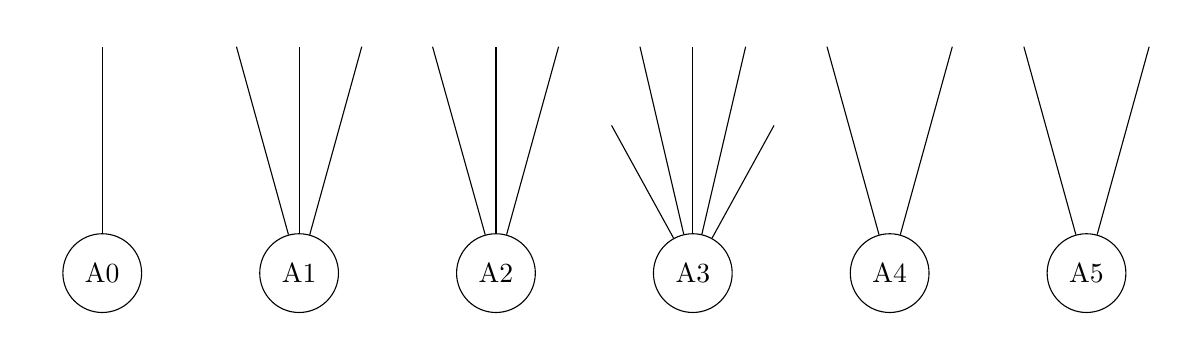
\begin{tikzpicture}
\node[state, minimum size=1cm](A0) at (0,0) {A0};
\node[state, minimum size=1cm](A1) at (2.5,0) {A1};
\node[state, minimum size=1cm](A2) at (5,0) {A2};
\node[state, minimum size=1cm](A3) at (7.5,0) {A3};
\node[state, minimum size=1cm](A4) at (10,0) {A4};
\node[state, minimum size=1cm](A5) at (12.5,0) {A5};

\node(B0) at (-0.83,3) {};
\node(B1) at (0,3) {};
\node(B2) at (0.83,3) {};
\node(B3) at (1.67,3) {};
\node(B4) at (2.5,3) {};
\node(B5) at (3.33,3) {};
\node(B6) at (4.16,3) {};
\node(B7) at (5,3) {};
\node(B8) at (5.83,3) {};
\node(B9) at (6.8,3) {};
\node(B9a) at (6.4,2) {};
\node(B10) at (7.5,3) {};
\node(B11) at (8.2,3) {};
\node(B11a) at (8.6,2) {};
\node(B12) at (9.17,3) {};
\node(B13) at (10,3) {};
\node(B14) at (10.83,3) {};
\node(B15) at (11.67,3) {};
\node(B16) at (12.5,3) {};
\node(B17) at (13.33,3) {};

%\draw[-] (A0) -- (B0);
\draw[-] (A0) -- (B1);
%\draw[-] (A0) -- (B2);
\draw[-] (A1) -- (B3);
\draw[-] (A1) -- (B4);
\draw[-] (A1) -- (B5);
\draw[-] (A2) -- (B6);
\draw[-] (A2) -- (B7);
\draw[-] (A2) -- (B8);
\draw[-] (A3) -- (B9);
\draw[-] (A3) -- (B9a);
\draw[-] (A3) -- (B10);
\draw[-] (A3) -- (B11);
\draw[-] (A3) -- (B11a);
\draw[-] (A4) -- (B12);
%\draw[-] (A4) -- (B13);
\draw[-] (A4) -- (B14);
\draw[-] (A5) -- (B15);
%\draw[-] (A5) -- (B16);
\draw[-] (A5) -- (B17);
\end{tikzpicture}
\caption{Example of six nodes with a Poisson degree distribution with mean 3.}
\label{fig:5.1}
\end{figure}

\begin{figure}
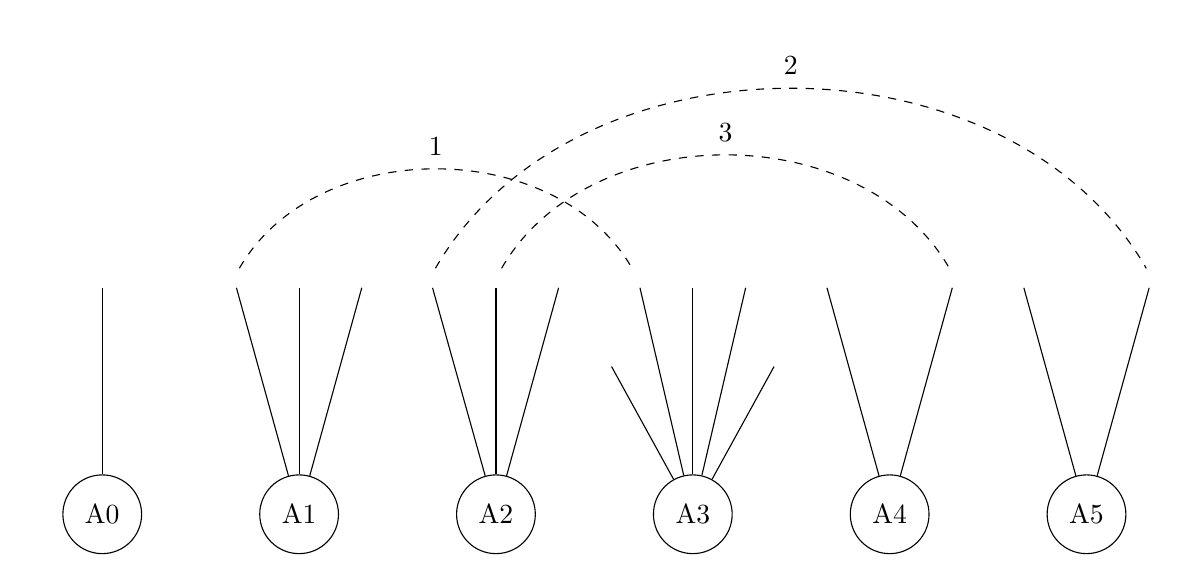
\begin{tikzpicture}
\node[state, minimum size=1cm](A0) at (0,0) {A0};
\node[state, minimum size=1cm](A1) at (2.5,0) {A1};
\node[state, minimum size=1cm](A2) at (5,0) {A2};
\node[state, minimum size=1cm](A3) at (7.5,0) {A3};
\node[state, minimum size=1cm](A4) at (10,0) {A4};
\node[state, minimum size=1cm](A5) at (12.5,0) {A5};

\node(B0) at (-0.83,3) {};
\node(B1) at (0,3) {};
\node(B2) at (0.83,3) {};
\node(B3) at (1.67,3) {};
\node(B4) at (2.5,3) {};
\node(B5) at (3.33,3) {};
\node(B6) at (4.16,3) {};
\node(B7) at (5,3) {};
\node(B8) at (5.83,3) {};
\node(B9) at (6.8,3) {};
\node(B9a) at (6.4,2) {};
\node(B10) at (7.5,3) {};
\node(B11) at (8.2,3) {};
\node(B11a) at (8.6,2) {};
\node(B12) at (9.17,3) {};
\node(B13) at (10,3) {};
\node(B14) at (10.83,3) {};
\node(B15) at (11.67,3) {};
\node(B16) at (12.5,3) {};
\node(B17) at (13.33,3) {};

%\draw[-] (A0) -- (B0);
\draw[-] (A0) -- (B1);
%\draw[-] (A0) -- (B2);
\draw[-] (A1) -- (B3);
\draw[-] (A1) -- (B4);
\draw[-] (A1) -- (B5);
\draw[-] (A2) -- (B6);
\draw[-] (A2) -- (B7);
\draw[-] (A2) -- (B8);
\draw[-] (A3) -- (B9);
\draw[-] (A3) -- (B9a);
\draw[-] (A3) -- (B10);
\draw[-] (A3) -- (B11);
\draw[-] (A3) -- (B11a);
\draw[-] (A4) -- (B12);
%\draw[-] (A4) -- (B13);
\draw[-] (A4) -- (B14);
\draw[-] (A5) -- (B15);
%\draw[-] (A5) -- (B16);
\draw[-] (A5) -- (B17);

\path[dashed](B3)edge[bend left=60]node[above=0.05cm]{1}(B9);
\path[dashed](B6)edge[bend left=60]node[above=0.05cm]{2}(B17);
\path[dashed](B7)edge[bend left=60]node[above=0.05cm]{3}(B14);
\end{tikzpicture}
\caption{Example of how the nodes in Figure \ref{fig:5.1} may begin to be paired up}
\label{fig:5.2}
\end{figure}

\begin{figure}
\begin{center}
\begin{tikzpicture}
\node[state, minimum size=1cm](A0) at (360/6: 4cm) {A0};
\node[state, minimum size=1cm](A1) at (2*360/6: 4cm) {A1};
\node[state, minimum size=1cm](A2) at (3*360/6: 4cm) {A2};
\node[state, minimum size=1cm](A3) at (4*360/6: 4cm) {A3};
\node[state, minimum size=1cm](A4) at (5*360/6: 4cm) {A4};
\node[state, minimum size=1cm](A5) at (360: 4cm) {A5};

\path(A5)edge[bend right=10](A1);
\path(A0)edge(A4);
\path(A3)edge[out=240,in=300,looseness=15](A3);
\path(A2)edge[bend left=10](A3);
%\path(A5)edge(A0);
\path(A5)edge[bend left=10](A1);
\path(A2)edge(A4);
\path(A1)edge(A3);
\path(A2)edge[bend right=10](A3);
%\path(A0)edge[bend left=10](A4);
\end{tikzpicture}
\end{center}
\caption{The complete random network of the nodes in Figure \ref{fig:5.1}}
\label{fig:5.3}
\end{figure}

Another requirement of the random network is that there are no loops or multiple edges. If there is a loop in a graph this means that there are two edges connected to the same node which have been paired up. This is undesirable since it makes no sense to have an individual who is their own neighbour since a person cannot infect nor be infected by themselves. However, during the generation of the random network loops are still possible if the two half edges chosen to be paired up are connected to the same node. If a graph has multiple edges then it means there is more than one edge connecting two individuals, which is undesirable since it would mean that there exists two individuals who are neighbours to each other twice, which would make no sense, either you are neighbours with someone or you aren’t. A graph which has no loops or multiple edges is called a ``simple” graph, so we need to generate the random network to be a simple graph. 

One way to make sure that the total number of half edges or the sum of the degrees is even is to repeatedly generate all of the degrees of the individuals in the population until the sum of the degrees $\sum_{k=1}^{N} d_i$ is even. In other words we require $ \frac{1}{2} \sum_{k=1}^{N} d_i \in \mathbb{N}$. Of course the sum of the degrees could be $0$ but this graph would be trivial and as a result not worth considering. Alternatively, if the sum of the degrees is odd then we can randomly erase a half edge, giving us the correct amount. If we choose to erase edges, then this solves the issue of loops and multiple edges since they can also just be erased. This new model is called the erased configuration model. However, in doing this there could create an issue. Let a random graph have prescribed degree distribution $F$. As outlined in \cite{bibbritton} the probability of randomly choosing a half edge which is connected to the node which has the maximum degree is not negligible, and by extension any node with degree $d_i>1$ has a positive probability of being connected to this node. As a result, if edges are erased then the degree of the nodes that were connected to these edges will decrease and the new degree distribution of the graph will converge to a distribution which is smaller than $F$. However, as long as the degree distribution has finite mean, then the new degree distribution converges to $F$ as the size of the population $N$ tends to infinity. The proof for this is not included in this report but can be found in \cite{bibbritton}. Since in this project we will only consider degree distributions with finite mean, this will not affect the configuration model.

\begin{figure}
\begin{center}
\begin{tikzpicture}
\node[state, minimum size=1cm](A0) at (360/6: 4cm) {A0};
\node[state, minimum size=1cm](A1) at (2*360/6: 4cm) {A1};
\node[state, minimum size=1cm](A2) at (3*360/6: 4cm) {A2};
\node[state, minimum size=1cm](A3) at (4*360/6: 4cm) {A3};
\node[state, minimum size=1cm](A4) at (5*360/6: 4cm) {A4};
\node[state, minimum size=1cm](A5) at (360: 4cm) {A5};

\path(A2)edge(A3);
%\path(A5)edge(A0);
\path(A5)edge(A1);
\path(A2)edge(A4);
\path(A1)edge(A3);
\path(A0)edge(A4);
\end{tikzpicture}
\end{center}
\caption{The erased model of Figure \ref{fig:5.3}}
\label{fig:erased}
\end{figure}

Another way to make sure that the random network has no loops or multiple edges is to repeat the algorithm which generates the random network until a graph is generated which is simple. This model is called the repeated model. The issue with the repeated model is that if it takes a number of attempts to obtain a simple graph then this graph might not be typical of the configuration model. For example, it might be the case that there is an unusually small number of edges since by chance there happen to be no multiple edges or loops. By extension this could mean the degrees of individuals is skewed so that individuals have unusually small degrees since the degrees are chosen at random. But as long as the prescribed degree distribution has finite second moment then the degree distribution in the repeated configuration converges to $F$ as the size of the population $N$ tends to infinity. The proof for this also not included in this report but is included in \cite{bibbritton}. During this project, when generating the random network, the model that is used in the erased configuration model.

\begin{figure}
\begin{center}
\begin{tikzpicture}
\node[state, minimum size=1cm](A0) at (360/6: 4cm) {A0};
\node[state, minimum size=1cm](A1) at (2*360/6: 4cm) {A1};
\node[state, minimum size=1cm](A2) at (3*360/6: 4cm) {A2};
\node[state, minimum size=1cm](A3) at (4*360/6: 4cm) {A3};
\node[state, minimum size=1cm](A4) at (5*360/6: 4cm) {A4};
\node[state, minimum size=1cm](A5) at (360: 4cm) {A5};

\path(A2)edge(A0);
\path(A0)edge(A4);
\path(A4)edge(A3);
\path(A3)edge(A2);
\path(A4)edge(A1);
\path(A4)edge(A5);
\end{tikzpicture}
\end{center}
\caption{The repeated model of the nodes in Figure \ref{fig:5.1}}
\label{fig:repeated}
\end{figure}

An alternative to thinking of the configuration model as a graph is to think of it as an adjacency matrix $A$. The matrix will be $N\times N$ and $A_{i,j}$ will take value $0$ if $i$ and $j$ are not connected, the value $1$ if there is one connection between $i$ and $j$, the value $2$ if there are two connections between $i$ and $j$, etc. This matrix is necessarily symmetrical since if there are $m$ connections between $i$ and $j$ then there are also $m$ connections between $j$ and $i$. Then the matrix for the erased configuration model $A’_{i,j}$ will have zero’s on the diagonal since there are no loops in the erased configuration model and it will be binary meaning that there all entries of the matrix are either $0$ or $1$ as all entries greater or equal to $1$ are made equal to $1$.

\subsubsection{Interpretting the random network} \label{subsub:5.1.3}

So now we know that the structure of the configuration model will depend on the size of the population, the prescribed degree distribution and the mean of the degree distribution. The random graph in Figure \ref{Po5 n100} is an erased random graph of $100$ individuals represented by nodes with a Poisson degree distribution with mean $5$. As we can see it is quite difficult to see much of what is going on and the graph looks quite chaotic, but we can see that the degrees of the individuals are quite concentrated about the mean of the degree distribution as there is only $1$ individual which degree $0$ and only a few individuals with degree $1$ which appear on the outskirts of the graph which is typical of the Poisson distribution as it has a light tail. If a probability distribution has a light tail then it has a tail which goes to zero more quickly than an exponential distribution, if it has a heavy tail then it has a tail which goes to zero slower than an exponential distribution \cite{bibbryson}. If we increase the size of the population but keep the degree distribution and the mean of the degree distribution the same as in Figure \ref{Po5 n100} then we get a graph similar to Figure \ref{Po5 n1000}. This is a graph of a population of $1000$ but still with a Poisson degree distribution with mean $5$. Now it is even less apparent of the structure of the random network since it is very busy and all the lines connecting the nodes merge together. We say that a graph looks busy if it is difficult to distinguish between connections between nodes. This means that it is difficult to see the structure of a random network unless the population is sufficiently small.

Figure \ref{Po10 n100} is a random network of a population of $100$ individuals with a Poisson degree distribution with mean $10$. Similar to before, since the degree distribution is the Poisson distribution, the degrees of individuals are quite concentrated about the mean of the degree distribution, so it is busier than Figure \ref{Po5 n100} as it is more difficult to distinguish between connections between individuals. Finally, in Figure \ref{Geom5 n100} the degree distribution of the random graph has been changed but the mean of the degree distribution and the population size have been kept the same. Here the random graph is of $100$ individuals with a Geometric degree distribution with mean $5$. The Geometric distribution has a much heavier tail than the Poisson distribution and this is reflected in Figure \ref{Geom5 n100} by the fact that the degrees of the individuals are not very concentrated around the mean of the distribution.  We can see this since there are a large number of individuals by themselves with degree $0$ or on the edge of the graph with $1$ neighbour and there a few individuals at the centre of the graph who have a large number of neighbours.


\begin{figure}
\begin{center}
\includegraphics[height=10cm, width=15cm]{/Users/christianpearce/Documents/MMath/Year 4/Dissertation/Dissertation writing/Po5 n100.jpg}
\end{center}
\caption{Graph of erased configuration model of 100 individuals with Poisson degree distribution with mean 5}
\label{Po5 n100}
\end{figure}

\begin{figure}
\begin{center}
\includegraphics[height=10cm, width=15cm]{/Users/christianpearce/Documents/MMath/Year 4/Dissertation/Dissertation writing/Po5 n1000.jpg}
\end{center}
\caption{Graph of erased configuration model of 1000 individuals with Poisson degree distribution with mean 5}
\label{Po5 n1000}
\end{figure}

\begin{figure}
\begin{center}
\includegraphics[height=10cm, width=15cm]{/Users/christianpearce/Documents/MMath/Year 4/Dissertation/Dissertation writing/Po10 n100.jpg}
\end{center}
\caption{Graph of erased configuration model of 100 individuals with Poisson degree distribution with mean 10}
\label{Po10 n100}
\end{figure}


\begin{figure}
\begin{center}
\includegraphics[height=10cm, width=15cm]{/Users/christianpearce/Documents/MMath/Year 4/Dissertation/Dissertation writing/Geom5 n100.jpg}
\end{center}
\caption{Graph of erased configuration model of 100 individuals with Geometric degree distribution with mean 5}
\label{Geom5 n100}
\end{figure}

\subsection{The SIS Epidemic} \label{subsub:5.2}

Now that the configuration model is defined, the SIS epidemic model can be defined and how it acts on a random network. First of all, the initial infectious individuals are chosen. As with the real epidemic, the SIS epidemic model consists of a series of events, either an infection of a susceptible individual or the recovery of an infectious individual occurring through time. However, whereas in the real epidemic some individuals can be infected through less contact with an infectious individual than others, and some individuals may recover at different rates than others, in the SIS model infections and recoveries are assumed to occur at constant rates. These rates will be denoted $\lambda$ and $\mu$ respectively. This assumption dramatically simplifies the infection dynamics of the mathematical model since if every individual had different infection and recovery rates then more data has to be taken into account when computationally simulating the mathematical model and could make it very difficult.

Since the infection and recovery rates are constant, this means that the rate at which an infectious individual infects a susceptible neighbour is described by a Poisson process \cite{bibandersson3}. Because this follows a Poisson process this also means that the infection times, which is the length of time an individual is infectious for, follows an exponential distribution with mean $1/ \mu$ and are independent of each other. As well, this means that the time until the next event is exponentially distributed with rate parameter equal to the total rate of the SIS epidemic at time $t$. The total rate of the SIS epidemic at time $t$ is the sum of the product of the infection rate $\lambda$ and the number of potential infections that could happen at time $t$ and the product of the recovery rate $\mu$ and the number of recoveries that could happen at time $t$. In other words, the total rate is the sum of the rates of every possible event that could occur at time $t$. As the number of potential events increases, so does the total rate meaning that the time until the next event occurs decreases. 


\subsection{The SIS Epidemic on a Random Network} \label{subsub:5.3}

Now we have rigorously defined both parts of the mathematical model separately we can simulate how they interact when combined.

The first thing is to choose the degree distribution for the configuration model and the population size. The most common discrete probability distribution is the Poisson distribution, so this is a sensible distribution with which to begin. Once a suitable random network has been generated then the initially infected individuals are chosen at random and we begin the epidemic. Since each individual has certain neighbours, they will only be infected by and infect these neighbours. We say that a susceptible individual with an infectious neighbour make up an SI pair. Define $T_i$ the time of the i'th event, then to find the time at which the next event will occur, a random variable is generated using the exponential distribution described above. This is then added to the current time, giving the time at which the next event occurs. To decide what the next event will be a random variable is chosen at random on the interval $[0,\phi(t)]$ where 

\begin{equation} \label{totalrate}
\phi(t) = \lambda \times\mbox{(no. SI pairs)} + \mu \times\mbox{(no. of infected individuals)}
\end{equation}

is the total rate of the epidemic at time $t$. This rate is not constant and will change throughout time depending on which infectious and susceptible individuals are infected at time $t$.  If the random variable is less than the product of the number of possible infections at time $t$ and the infection rate then the next event will be an infection, else the next event will be a recovery. 

In the first case, the susceptible individual who will be infected then needs to be chosen. To do this we take all SI pairs in the population and choose one uniformly at random. This susceptible individual in this pair then becomes infectious and the cycle begins again. In the second case, the infectious individual who will recover and return to a susceptible state needs to be chosen. To do this we take all of the infectious individuals and choose one uniformly at random, this individual then returns to a susceptible state and the cycle begins again. This essentially means that the next event is chosen from all possible events at random. This goes on for a pre-determined number of events, after each event recording the number of infected individuals and then stop the simulation.

Figure \ref{1 SIM lambda 1 mu 1} is a typical simulation for a population of $100$ people, with a Poisson prescribed degree distribution with mean $5$, and infection rate and recovery rate given by $\lambda=1$ and $\mu=1$ respectively. The simulation plots the length of the simulated epidemic which is $1000$ events which may be infections or recoveries, against the number of infected individuals at the time of each event. As we can see, for these parameters the epidemic takes off and appears to “level off”, yet there is still some randomness in the way the way the number of infected individuals progresses. 

\begin{figure}
\begin{center}
\includegraphics[height=10cm, width=15cm]{/Users/christianpearce/Documents/MMath/Year 4/Dissertation/Dissertation writing/1 SIM lambda 1 mu 1.jpg}
\end{center}
\caption{1 simulation of the SIS epidemic on a random network with Poisson degree distribution with mean 5, population size 100, 10 individuals initially infected, $\lambda$=1, $\mu$=1.}
\label{1 SIM lambda 1 mu 1}
\end{figure}

However, if we simulate the epidemic for the same number of events multiple times and take the mean value of the times of the $i$’th event where $i \in \{1,2,…,Q\}$, where $Q$ is the number of events the simulation runs for, and the mean number of infected individuals that are infected at the time of each event and plot them then we can see the mean behaviour of the epidemic. This means that when we plot the mean epidemic we are plotting the expected time of the i'th event  against the expected number of infectious individuals at the expected time of the i'th event given by \eqref{E[I(E[T_n])]}.

\begin{equation}\label{E[I(E[T_n])]}
E[I(E[T_i])]\,\,\,\,\,\,\,\,\,\,\,\,\,\,\, i \in \{1,2,...,Q\}
\end{equation}


Figure \ref{10 SIM lambda 1 mu 1} shows $10$ simulations of the SIS epidemic in grey for the same parameters as Figure \ref{1 SIM lambda 1 mu 1} and the mean of these simulations in blue. For each simulation a new random network is generated, and new initial infected individuals are chosen. As we can see the mean behaviour of the simulations is less erratic than a single simulation and the mean behaviour of the epidemic is clearer. This behaviour is similar to the behaviour of the spread of computer viruses found in \cite{bibkephart}.

If we simulate the epidemic a large number of times and take the mean event times and mean number of infected individuals at the time of the $i$’th event, then the mean behaviour of the epidemic becomes much smoother and looks almost deterministic, so we can determine the behaviour of the epidemic more precisely. Figure \ref{SIM 100 Po5 lambda 1 mu 1} shows the mean behaviour of $100$ simulations of the epidemic with the same parameters as the simulations in Figure \ref{10 SIM lambda 1 mu 1} and Figure \ref{1 SIM lambda 1 mu 1} in grey and the mean of these simulations in blue. Again, the individual simulations are given by the grey lines however since the epidemic has been simulated a large number of times it becomes very difficult to see the how the individual simulations behave.

\begin{figure}
\begin{center}
\includegraphics[height=10cm, width=15cm]{/Users/christianpearce/Documents/MMath/Year 4/Dissertation/Dissertation writing/10 SIM lambda 1 mu 1.jpg}
\end{center}
\caption{10 simulations of the SIS epidemic on a random network with Poisson degree distribution with mean 5, population size 100, 10 individuals initially infected, $\lambda$=1, $\mu$=1 (grey) and their mean (blue).}
\label{10 SIM lambda 1 mu 1}
\end{figure}

\begin{figure}
\begin{center}
\includegraphics[height=10cm, width=15cm]{/Users/christianpearce/Documents/MMath/Year 4/Dissertation/Dissertation writing/SIM 100 Po5 lambda 1 mu 1.jpg}
\end{center}
\caption{100 simulations of the SIS epidemic on a random network with Poisson degree distribution with mean 5, population size 100, 10 individuals initially infected, $\lambda$=1, $\mu$=1 (grey) and their mean (blue).}
\label{SIM 100 Po5 lambda 1 mu 1}
\end{figure}

\subsection{Properties of the mean epidemic}
\label{subsub:5.4}

\subsubsection{Overwiew} \label{subsub:5.4.1}

From the mean behaviour of the epidemic we are able to see some interesting characteristics of its behaviour. Firstly, it tells us whether the epidemic takes off or not. What is meant by this is that an epidemic does one of two things; either it takes off and the infection becomes established in the population and the number of infectious individuals increases or the epidemic crashes, meaning the infection goes extinct quickly and the number of infected individuals goes to $0$ quickly. If the mean number of infected individuals $I(t)$ goes to $0$ as $t$ gets large, then this means that for every simulation the infection becomes extinct. From equation \eqref{takeoffeq}, if the number of simulations is large and the mean number of infected individuals $I(t)$ still goes to $0$ as $t$ gets large, then the probability of the epidemic taking off is $0$. Conversely, if the mean number of infectious individuals increases with $t$ then it is apparent that the probability of the epidemic taking off is strictly positive. By adjusting the parameters and the degree distribution of the mathematical model, we can see for which parameters the epidemic takes off and when it goes extinct.

\begin{equation} \label{takeoffeq}
\begin{split}
I(t)=I(t)\vert\, \mbox{epidemic geos extinct} \times P(\mbox{epidemic goes extinct}) +\\
I(t)\vert\, \mbox{epidemic takes off} \times P(\mbox{epidemic takes off})
\end{split}
\end{equation}

This number of events is chosen to be sufficiently large number so that the simulated epidemic runs for long enough so that we can see whether the epidemic takes off or goes extinct but not too large since once this behaviour can be identified there is no point in the simulation running further for a long time.

\subsubsection{Stable states of the mean epidemic} \label{subsub:5.4.2}

Another characteristic of the epidemic that can be explored by looking at the mean number of infectious individuals over time is the proportion of the population that is comprised of infectious individuals the epidemic settles at. If the epidemic takes off, because the population that the epidemic is on is closed, the number of infectious individuals will increase and then level off, reaching a steady state. This is not a steady state in the sense that the epidemic will not move from this state so is not a fixed point, more the value that the mean settles at in the time frame that the simulations run for. This value of $I(t)$ will depend on the parameters of the epidemic and the structure of the configuration model. Given that the epidemic takes off we could also look at how quickly the epidemic reaches this steady state, which will also depend on the structure of the configuration model and the parameters of the SIS epidemic.

It is worth noting however that the epidemic will always have one fixed point at $I(t)=0$ since if there are no infectious individuals in the population there can be no infections or recoveries so at the time of the next event and, in fact every event after that there will remain the same number of infectious individuals in the population. By fixed point we mean that if $I(t)=\alpha$ then $\alpha$ is a fixed point if after the next event then the value of $I(t)$ is $\alpha$ with probability $1$. It is also worth noting that since the simulations of the epidemic are random then as $t \rightarrow \infty$, there will inevitably be a sufficiently large fluctuation that will cause the epidemic will go extinct. This is because if there are $n$ infectious individuals in the population there is a positive probability that the next $n$  events are all recoveries i.e $P\{\mbox{next n events are recoveries}\}>0$ so this event must occur at some point as $t \rightarrow \infty$ and when it does, the value of $I(t)$ will hit $0$ and as $I(t)=0$ is a fixed point of the random process, the value of $I(t)$ will stay at $0$. 

By the law of large numbers, the number at which the mean number of infected individuals $I(t)$ reaches a level of stability is the point at which the rate of infection is equal to the rate of recovery i.e.

\begin{equation}\label{equilibrium}
\mu\times\mbox{(number of infected individuals)}=\lambda\times\mbox{(number of SI pairs)}
\end{equation}

This means that if $\mu=\lambda$ then, at this point the mean number of susceptible neighbours that an infectious individual has is $1$. This also mean that the number of infected individuals is given by

\begin{equation}
\mbox{(number of infected individuals)}=\frac{\lambda}{\mu}\times\mbox{(number of SI pairs)}
\end{equation}

Another way of thinking about this is in terms of flipping a coin. Similar to flipping a coin, the events in the random process of the epidemic can have have two outcomes; either an infection occurs or a recovery occurs, if we flip a coin the outcome will either be heads or tails. First define $X_0=0$ and flip a coin $N$ times and say for $\{X_n:n\geq1\}$ $X_n=1$ if the coin land on heads and $X_n=-1$ if the coin lands on tails. Equivalently we have $P(X_n=1)=\frac{1}{2}$ and $P(X_n=-1)=\frac{1}{2}$. Now define $Z_n=X_0+X_1+...+X_n$. Since $E[X_n]=0$ then $E[Z_n]=0, \forall n\geq 1$. 

Now if we consider \eqref{equilibrium}, define $X_0$ to be the value of $I(t)$ at which we first have \eqref{equilibrium} and we have $P(\mbox{next event is an infection})=P(\mbox{next event is a recovery})=\frac{1}{2}$, two events both with probability $\frac{1}{2}$. Define $P(X_n=1)=P(\mbox{next event is an infection})$ $P(X_n=-1)=P(\mbox{next event is a recover})$ and define $Z_n$ as before. Note that if the next event is an infection then the value of $I(t)$ will increase but will mean that 

\begin{equation}
\mu\times\mbox{(number of infected individuals)}>\lambda\times\mbox{(number of SI pairs)}
\end{equation}

\noindent
so it is more likely that the next event lowers the value of $I(t)$. On the other hand if we have the equality in \eqref{equilibrium} and a recovery occurs then the value of $I(t)$ decreases but then 

\begin{equation}\label{infectionlikely}
\mu\times\mbox{(number of infected individuals)}<\lambda\times\mbox{(number of SI pairs)}
\end{equation}
\noindent
so it is more likely for the next event to increase the value of $I(t)$. This is equivalent to saying that if there have been more heads than tails the probability of tails increases or vice-versa, and so the probabilities of an infection or a recovery occurring get pushed back towards $\frac{1}{2}$. This means that $E[Z_n]=E[X_0+X_1+...+X_n]=I(t)$ as $t \rightarrow \infty$.

This means that if $\lambda$ increases then we should expect that the mean number of infectious individuals the epidemic finds stability at should increase. Also, that if $\mu$ increase then we should expect that this number should decrease. As well, if the value of $\lambda$ and $\mu$ both change, whether they increase or decrease but their ratio stays the same then the number of infectious individuals at which the epidemic finds stability should stay the same.

\subsubsection{Probability of extinction of the mean epidemic} \label{subsub:5.4.3}

Initially, it will be more likely for an infection to occur than a recovery if we have \eqref{infectionlikely} or

\begin{equation}
\mbox{(number of infected individuals)}<\frac{\lambda}{\mu}\mbox{(number of SI pairs)}
\end{equation}
\noindent
since the next event is chosen uniformly from all possible events. Since the initial number of infected individuals is chosen, it will be given by a constant $c$. So, if the population is sufficiently large then we can assume the initial infectious individuals are not neighbours of one another so the number of SI pairs will approximately be the product of the number of infectious individuals and the mean degree of the population. And so, we have

\begin{equation}
c<\frac{\lambda}{\mu}c\overline{k}
\end{equation}

\noindent
which can be simplified to 

\begin{equation}
\frac{\mu}{\lambda}<\overline{k}
\label{extincteq}
\end{equation}

\noindent
where $\overline{k}$ is the mean of the degree distribution.

This means that if $\frac{\mu}{\lambda}<\overline{k}$ then it is more likely than not that the epidemic will take off and become established in the population. Conversely, if $\frac{\mu}{\lambda}>\overline{k}$ then it is more likely that the epidemic will initially have negative trend and become extinct. This is another thing that we will be able to see from the mean behaviour of simulations. This also means that if we keep $\overline{k}$ constant, as $\frac{\mu}{\lambda}$ increases then it becomes more likely that the epidemic will quickly become extinct. If we consider the other variable we can change in \eqref{extincteq}, the mean of the degree distribution, then we can see that if we keep $\frac{\mu}{\lambda}$ constant and increase $\overline{k}$ then it is more likely that the epidemic takes off and becomes established in the population and if $\overline{k}$ is decreased then it is more likely that the epidemic goes extinct quickly. If the mean of the simulations tends to $0$ then this means all of the simulations have gone extinct so we would expect that in this case $\frac{\mu}{\lambda}$ is far larger than $\overline{k}$. This also means that whether the mean epidemic takes off or goes extinct will not depend on the epidemic threshold. The epidemic threshold is the proportion of susceptible individuals in the population required for an epidemic to take off. As far as my literature research has gone this property of the epidemic has not been previously documented.

\subsubsection{The rate at which the mean epidemic finds stability} \label{subsub:5.4.4}

Another characteristic of the mean behaviour of the epidemic we may want to consider is how quickly the epidemic appears to level off and stabilise. There are more than one factors contributing to this. Firstly, the time taken for the epidemic to stabilise will be shorter in an epidemic where there are more possible infections at time $t$ as opposed to an epidemic where there are less possible infections at time $t$. In other words the time taken for an epidemic to stabilise will be shorter if a larger proportion of the total rate of the epidemic at time $t$ \eqref{totalrate} is taken up by the number of SI pairs, meaning an infection is more likely. Secondly, the time taken for the epidemic to stabilise will be less if the time between events is shorter meaning that the total rate of the epidemic at time $t$ \eqref{totalrate} must be greater. 

In the first case, as with whether it is more likely that an epidemic goes extinct or takes off, an epidemic will take off faster if the probability of choosing the next event to be an infection as opposed to a recovery is greater. This means that we would need the proportion of the total rate of the epidemic which is given by the number of possible infections to be larger or the proportion of the total rate of the epidemic given by the possible number of recoveries to be smaller. The first way we could do this is to increase $\lambda$ or decrease $\mu$ since this would make the probability of choosing a point in the interval in the total rate of the epidemic which would mean that the next event is an infection more likely, or it would make choosing a point in the interval in the total rate of the epidemic which would mean that the next event would be a recovery less likely.

We could also seek to increase the number of SI pairs or decrease the number of possible recoveries. However, if we decrease the number of possible recoveries then this would eliminate an infectious individual which could also remove multiple SI pairs form the epidemic. On the other hand, if we increase the number of SI pairs then this would increase the number of events that could cause an infection and increase the probability of choosing a point in the interval of the total rate of the epidemic which would mean that the next event is an infection. The first way we could do this is to increase the number of infected individuals, we could do this by choosing a larger proportion of the population to be initially infected. However, if this is chosen to be too high then the population will become saturated with infected individuals and the number of recoveries could become dominant. As well as this, it would mean that the epidemic would start out with a considerable proportion of the individuals in the population already infected and this is unrealistic since the epidemic has to start with a small proportion of the population being infectious. This also means that if the epidemic takes off, we should expect that as the number of infected individuals increases then the rate at which the number of infected individuals increases also increases. 

Alternatively, we could increase the number of susceptible neighbours the infected individuals have. This can be done by increasing the mean of the degree distribution since, if the average number of neighbours an individual has increases then the number of susceptible neighbours an individual has is likely to increase as well, and as a result the number of SI pairs will increase. So, given that the epidemic takes off, if we increase the mean of the prescribed degree distribution of the configuration model then we would expect the number of infectious individuals to increase more quickly. Another way to increase the number of SI pairs is to change the prescribed degree distribution. If the degree distribution has a light tail such as a Poisson distribution, then all of the degrees will be quite concentrated around the mean whereas, if the prescribed degree distribution has a heavy tail, such as a Geometric distribution, then there will be individuals with a more extreme number of neighbours. Therefore, this could mean that the number of susceptible neighbours an infectious individual has, has the potential to be higher, which in turn would increase the number of SI pairs.

The other factor that could mean that the time the epidemic takes to reach a level of stability is shorter is the time it takes for the next event to occur. In other words, if events happen in quicker succession then the epidemic will reach the level of stability in less time. The time until the next event is determined by a random variable with exponential distribution with rate parameter equal to the total rate of the epidemic.  As previously stated the total rate of the epidemic at time $t$ is the sum of the product of the infection rate $\lambda$ and the number of potential infections that could happen at time $t$ and the product of the recovery rate $\mu$ and the number of infections that could happen at time $t$. So, if this increases then the time until the next event will decrease. This means we can either increase $\mu$ or $\lambda$ and this would increase the total rate of the epidemic. As well as this it could be increased by increasing the number of infected individuals or the number of SI pairs. As discussed above we could increase the number of infected individuals by choosing a larger proportion of the population to be initially infectious however this is unrealistic when considered in terms of a real epidemic so this will not be considered. We could however try to increase the number of SI pairs to increase the total rate of the epidemic. As before we could either increase the mean of the prescribed degree distribution or change the degree distribution to a degree distribution which has a heavier tail.

\subsubsection{Summary of properties of the mean epidemic} \label{subsub:5.4.5}

To summarise, we are looking at the mean behaviour of the epidemic for a given set of parameters. The parameters of the epidemic are the number of individuals in the population $N$, the prescribed degree distribution of the configuration model and the mean of the degree distribution which we will denote $\overline{k}$, the number of initial infectious individuals $c$, the infection rate $\lambda$ and the recovery rate $\mu$. The characteristics of the mean behaviour of the epidemic that are of interest are whether the epidemic is likely to take off or quickly become extinct, if the epidemic takes off, the approximate number of infectious individuals when the epidemic reaches a level of stability and the rate at which it reaches this level of stability.

We should expect that whether the epidemic takes off or quickly becomes extinct will depend on the ratio of $\lambda$ and $\mu$ and the mean value of the degree distribution $\overline{k}$. The number of infectious individuals in the population when the epidemic reaches a level of stability should also be proportional to $\frac{\mu}{\lambda}$ and the mean value of the degree distribution $\overline{k}$. We also expect that the rate at which the epidemic reaches this level of stability should be proportional to the proportion of initially infectious individuals, the values of $\lambda$ and $\mu$ and the probability density function of the prescribed degree distribution and the mean $\overline{k}$, of the degree distribution. It is also possible that the mean behaviour of the epidemic may depend on the size of the population $N$ since the mathematical model assumes that $N \rightarrow \infty$.

Since it is the mean behaviour of the SIS epidemic on the random network that is of interest, the simulations are run multiple times and then the mean times of the i’th event and the mean number of infected individuals at the i'th event are calculated, which can then be plotted against each other. The mean behaviour of the SIS epidemic is the thing of interest because this tells us a few characteristics of the epidemic. Firstly, it tells us whether the epidemic takes off or not. What is meant by this is that an epidemic does one of two things; either it takes off and the infection becomes established in the population and the number of infectious individuals increases or the infection goes extinct quickly and the number of infectious individuals goes to $0$ quickly. If the mean number of infected individuals $I(t)$ at time $t$ goes to $0$ as $t$ gets large then this means that for every simulation the infection goes extinct. If the number of simulations is large and the mean number of infected individuals $I(t)$ still goes to $0$ as $t$ gets large, then the probability of the epidemic taking off is $0$. Conversely, if the mean number of infectious individuals increases with $t$ then it is apparent that the probability of the epidemic taking off is strictly positive. By adjusting the parameters and the degree distribution of the mathematical model, we can see for which parameters the epidemic takes off and when it goes extinct.

Another characteristic of the epidemic that can be explored by looking at the mean number of infectious individuals over time is the proportion of the population that is comprised of infectious individuals the epidemic settles at. If the epidemic takes off, because the population that the epidemic is on is closed, the number of infectious individuals will increase and then “level off”, reaching a steady state. This is not a steady state in the sense that the epidemic will not move from this state, more the value that the mean settles at in the time frame that the simulations run for. This value will depend on the parameters of the epidemic and the structure of the configuration model. Given that the epidemic takes off we could also look at how quickly the epidemic reaches this steady state, which will also depend on the structure of the configuration model and the parameters of the SIS epidemic.

\subsection{Results of the simulations of the mean epidemic}
\label{subsub:5.5}

\subsubsection{Results of changing the scale of the population of the epidemic} \label{subsub:5.5.1}

Beginning with Figure \ref{SIM 100 Po5 lambda 1 mu 1} which is of the mean of $100$ simulations of the SIS epidemic on a random network of $100$ individuals with $10$ of them being initially infectious, with Poisson degree distribution with mean $\overline{k}=5$, infection rate $1$ and recovery rate $1$ as a starting point, we can see that the mean epidemic takes off, so the probability of an epidemic taking off is positive. We can also see that the mean epidemic reaches a level of stability when the number of infectious individuals is around $75$ out of $100$ individuals. As well, it reaches this level of stability at around time $2$.

Using $100$ individuals may seem like a small population size, especially since many of the assumptions of the SIS epidemic and the configuration model assume that the population size is large, and $100$ individuals may not be considered large. So, we may want to know how much changing the population size to be much larger will change the mean behaviour of the epidemic. In Figure \ref{n1000 SIM 100 Po5 lambda 1 mu 1} the parameters and the degree distribution have been kept the same as in Figure \ref{SIM 100 Po5 lambda 1 mu 1} however, now using a much larger population of $1000$ individuals. As we can see the mean epidemic still takes off and reaches a level of stability when approximately $75\%$ of the individuals in the population are infectious. The mean epidemic also reaches this level of stability around the same time. The only significant change is that the mean epidemic seems a lot smoother and looks more deterministic. This is because when the population is larger the contribution of gaining or losing one infectious individual is smaller overall. This means that we can say that a population of $100$ individuals is sufficiently large to see the behaviour of the mean epidemic. As well, even though the mean epidemic using a population of $1000$ individuals reaches a level of stability at the same time, since there are more individuals in the population, the total rate of the epidemic is higher and so takes more events to reach this level of stability. Simulating $100$ simulations for a much larger number of events and for a much larger population takes much longer to simulate, so since using a population of $100$ individuals is sufficiently large that we can see the mean behaviour of the epidemic and does not change significantly  when the population size is increased, we will continue to investigate the mean behaviour of the epidemic using a population of $100$ individuals for the remainder of this report.

\begin{figure}
\begin{center}
\includegraphics[height=10cm, width=15cm]{/Users/christianpearce/Documents/MMath/Year 4/Dissertation/Dissertation writing/n1000 SIM 100 Po5 lambda 1 mu 1.jpg}
\end{center}
\caption{Mean of 100 simulations of the SIS epidemic on a random network with Poisson degree distribution with mean 5, population size 1000, 100 individuals initially infected, $\lambda$=1, $\mu$=1.}
\label{n1000 SIM 100 Po5 lambda 1 mu 1}
\end{figure}

\subsubsection{Results of changing the infection and recovery rates} \label{subsub:5.5.2}

Now consider the change to the mean behaviour of the epidemic if we change the parameters of the epidemic: the infection rate $\lambda$ and the recovery rate $\mu$. In Figure \ref{SIM 100 Po5 lambda 10 mu 1} the parameters and degree distribution of the configuration model have been kept the same as in Figure \ref{SIM 100 Po5 lambda 1 mu 1} except the infection rate $\lambda$ has been changed from $1$ to $10$. As we can see, the mean epidemic still takes off as expected and reaches a level of stability when the number of infectious is much greater, now around $95$ of the $100$ individuals are infectious. As well, the mean epidemic reaches this level of stability in a much shorter time, at approximately time $0.25$ which we also expected. Suppose instead now we changed the recovery rate as opposed to the infection rate. In Figure \ref{SIM 100 Po5 lambda 1 mu 10} the degree distribution and parameters have been kept the same as in Figure \ref{SIM 100 Po5 lambda 1 mu 1} but the recovery rate $\mu$ has been changed from $1$ to $10$. Now the mean epidemic tends to $0$, this is because all of the simulated epidemics have died out. This shows that in the case that the value of the recovery rate $\mu$ becomes large in comparison to the infection rate $\lambda$ then it is far more likely for the epidemic to go extinct quickly.

\begin{figure}
\begin{center}
\includegraphics[height=10cm, width=15cm]{/Users/christianpearce/Documents/MMath/Year 4/Dissertation/Dissertation writing/SIM 100 Po5 lambda 10 mu 1.jpg}
\end{center}
\caption{Mean of 100 simulations of the SIS epidemic on a random network with Poisson degree distribution with mean 5, population size 100, 10 individuals initially infected, $\lambda$=10, $\mu$=1.}
\label{SIM 100 Po5 lambda 10 mu 1}
\end{figure}

\begin{figure}
\begin{center}
\includegraphics[height=10cm, width=15cm]{/Users/christianpearce/Documents/MMath/Year 4/Dissertation/Dissertation writing/SIM 100 Po5 lambda 1 mu 10.jpg}
\end{center}
\caption{Mean of 100 simulations of the SIS epidemic on a random network with Poisson degree distribution with mean 5, population size 100, 10 individuals initially infected, $\lambda$=1, $\mu$=10.}
\label{SIM 100 Po5 lambda 1 mu 10}
\end{figure}

What if the values of the infection rate $\lambda$ and the recovery rate $\mu$ are both changed but their ratio now stays the same? In Figure \ref{SIM 100 Po5 lambda 10 mu 10} the degree distribution of the configuration model has been kept the same as in Figure \ref{SIM 100 Po5 lambda 1 mu 1} but the value of $\lambda$ and $\mu$ have both been increased to $10$, keeping the ratio of $\frac{\lambda}{\mu}$ the same. Much in the same way as Figure \ref{SIM 100 Po5 lambda 1 mu 1} the mean epidemic still takes off and reaches a level of stability at approximately the same number of infectious individuals, however, it reaches this level of stability at a much earlier time, at around time $0.2$. This is what we expected since if the infection and recovery rates are both much larger, then the total rate of the epidemic will be greater. In fact in this case, the values of $\lambda$ and $\mu$ are increased by a factor of $10$ so the total rate of the epidemic will have also increased by a factor of $10$, so it makes intuitive sense that the rate at which the mean epidemic reached a level of stability is a tenth of the time it took for the mean epidemic in Figure \ref{SIM 100 Po5 lambda 1 mu 1} to reach a level of stability.

\begin{figure}
\begin{center}
\includegraphics[height=10cm, width=15cm]{/Users/christianpearce/Documents/MMath/Year 4/Dissertation/Dissertation writing/SIM 100 Po5 lambda 10 mu 10.jpg}
\end{center}
\caption{Mean of 100 simulations of the SIS epidemic on a random network with Poisson degree distribution with mean 5, population size 100, 10 individuals initially infected, $\lambda$=10, $\mu$=10.}
\label{SIM 100 Po5 lambda 10 mu 10}
\end{figure}

\subsubsection{Results of changing the mean of the prescribed degree distribution} \label{subsub:5.5.3}

Now we have considered how a change in the parameters of the epidemic influences the mean behaviour of the epidemic, we can consider how changing the structure of the configuration model: the prescribed degree distribution and the parameters of the prescribed degree distribution, influences the mean behaviour of the epidemic. First of all, consider the case where the mean is increased. In Figure \ref{SIM 100 Po10 lambda 1 mu 1} the population size and the values of $\lambda$ and $\mu$ have been kept the same as in Figure \ref{SIM 100 Po5 lambda 1 mu 1}. The degree distribution has also been kept the same as in Figure \ref{SIM 100 Po5 lambda 1 mu 1}, but the mean has been increased from $5$ to $10$. We can see that the mean epidemic still takes off which is what we expected and that the proportion of the population that is infectious when the mean epidemic reaches a level of stability is higher. This may be because if the mean number of neighbours an individual has is higher then, there will be more total links between individuals and so early in the epidemic more neighbours of infectious individuals will be susceptible and so the number of SI pairs will be greater. This means that more individuals will have to be infectious before the number of infectious individuals and the number of SI pairs become approximately equal. As well as this, the mean epidemic takes less time to reach a level of stability, which could be because the number of SI pairs in the epidemic is greater, so the total rate of the epidemic is greater, which is what was expected.

\begin{figure}
\begin{center}
\includegraphics[height=10cm, width=15cm]{/Users/christianpearce/Documents/MMath/Year 4/Dissertation/Dissertation writing/SIM 100 Po10 lambda 1 mu 1.jpg}
\end{center}
\caption{Mean of 100 simulations of the SIS epidemic on a random network with Poisson degree distribution with mean 10, population size 100, 10 individuals initially infected, $\lambda$=1, $\mu$=1.}
\label{SIM 100 Po10 lambda 1 mu 1}
\end{figure}

Conversely, if the mean of the degree distribution is decreased while keeping the degree distribution and the parameters of the epidemic the same as in Figure \ref{SIM 100 Po5 lambda 1 mu 1} then, as seen in Figure \ref{SIM 100 Po2 lambda 1 mu 1} the mean epidemic takes off but takes much longer to reach a level of stability and when it does reach a level of stability, the proportion of infectious individuals in the population is much lower than in Figure \ref{SIM 100 Po5 lambda 1 mu 1}. The mean epidemic reaches a level of stability when approximately $30$ of the $100$ individuals in the population are infectious and reaches it at around time $8$. This is as expected since near the start of the epidemic if the individuals have a smaller degree on average there will be fewer total connections between individuals and as a result, the number of susceptible neighbours of infectious individuals will be fewer, meaning the total rate will be less. Also, since there are fewer SI pairs, the number of infectious individuals when the number of infectious individuals and the number of SI pairs become approximately equal will be less. The mean epidemic also still takes off, meaning that most of the time, for these parameters the epidemic will take off.

\begin{figure}
\begin{center}
\includegraphics[height=10cm, width=15cm]{/Users/christianpearce/Documents/MMath/Year 4/Dissertation/Dissertation writing/SIM 100 Po2 lambda 1 mu 1.jpg}
\end{center}
\caption{Mean of 100 simulations of the SIS epidemic on a random network with Poisson degree distribution with mean 2, population size 100, 10 individuals initially infected, $\lambda$=1, $\mu$=1.}
\label{SIM 100 Po2 lambda 1 mu 1}
\end{figure}

\subsubsection{Results of changing the ratio of $\frac{\mu}{\lambda}=\overline{k}$} \label{subsub:5.5.5}

So far when we have changed the values of the mean value of the degree distribution, the infection rate and the recovery rate, we have not considered how the behaviour of the mean epidemic might change if we adjusted these parameters so that $\frac{\mu}{\lambda}>\overline{k}$ as discussed in Section \ref{subsub:5.4}. In Figure \ref{SIM 100 Po2 lambda 1 mu 3} the parameters have been kept the same as in Figure \ref{SIM 100 Po5 lambda 1 mu 1}, except $\mu$ has been changed from $1$ to $3$ and $\overline{k}$ has been changed from $5$ to $2$ so that $\frac{\mu}{\lambda}>\overline{k}$. Now we can see that the mean epidemic goes extinct quickly which is what we expected.

\begin{figure}
\begin{center}
\includegraphics[height=10cm, width=15cm]{/Users/christianpearce/Documents/MMath/Year 4/Dissertation/Dissertation writing/SIM 100 Po 2 lambda 1 mu 3.jpg}
\end{center}
\caption{Mean of 100 simulations of the SIS epidemic on a random network with Poisson degree distribution with mean 2, population size 100, 10 individuals initially infected, $\lambda$=1, $\mu$=3.}
\label{SIM 100 Po2 lambda 1 mu 3}
\end{figure}

Furthermore, the parameters can be changed so that the ratio of $\mu$ to $\lambda$ is equal to the mean of the degree distribution i.e. $\frac{\mu}{\lambda}=\overline{k}$. This could reveal some interesting behaviour of the mean epidemic since this seems to be the turning point at which the mean epidemic moves from quickly becoming extinct to taking off and becoming established in the population. There are then two cases that need to be considered, either the mean of the prescribed degree distribution is large and is equal to $\frac{\mu}{\lambda}$ or it is small and is equal to $\frac{\mu}{\lambda}$. In these cases, the size of the infection and recovery rates should not matter as long as their ratio is equal to $\overline{k}$ since it has already been established that the size of these parameters does not affect whether or not the mean epidemic takes off or not, merely the rate at which it does so.

In Figure \ref{SIM 100 Po3 lambda 4 mu 12}, the degree distribution has been kept as a Poisson distribution, however, the mean has been decreased from $5$ to $3$ and the values of $\lambda$ and $\mu$ have been changed to $4$ and $12$ respectively. The mean epidemic now decreases in size as time goes on and does approach $0$. This indicates that all of the simulations go extinct. Similarly, in Figure \ref{SIM 100 Po8 lambda 1 mu 8} the degree distribution has been kept as a Poisson distribution however the mean has been increased to $8$ and the values of $\lambda$ and $\mu$ have been changed to $1$ and $8$ respectively, and now we can see that the number of infectious individuals in mean epidemic decreases in size and $I(t) \rightarrow 0$. This means that in this case as well all of the simulations eventually go extinct.

To see why this happens we can look at the individual simulations in these cases. In Figures \ref{SIM 100 Po3 lambda 4 mu 12 sim} and \ref{SIM 100 Po8 lambda 1 mu 8 sim} we can see that in these cases all of the simulations  go extinct but some go extinct quickly and and some appear to take off and become established in the population before going extinct later on. The value of $I(t)$ at which these simulations find a level of stability is fairly low so it does not appear that these simulations are taking off but this is what is happening. The reason that all of the simulations eventually go extinct is that because the simulations are random processes so there are constant fluctuations in the value of $I(t)$, and at some point in time because the value of $I(t)$ at which these simulations find a level of stability is sufficiently close to $0$ that there will eventually be a fluctuation sufficiently large that $I(t)$ hits $0$. This is in line with our prediction from Section \ref{subsub:5.4.2}.

\begin{figure}
\begin{center}
\includegraphics[height=10cm, width=15cm]{/Users/christianpearce/Documents/MMath/Year 4/Dissertation/Dissertation writing/SIM 100 Po3 lambda 4 mu 12.jpg}
\end{center}
\caption{Mean of 100 simulations of the SIS epidemic on a random network with Poisson degree distribution with mean 3, population size 100, 10 individuals initially infected, $\lambda$=4, $\mu$=12.}
\label{SIM 100 Po3 lambda 4 mu 12}
\end{figure}

\begin{figure}
\begin{center}
\includegraphics[height=10cm, width=15cm]{/Users/christianpearce/Documents/MMath/Year 4/Dissertation/Dissertation writing/SIM 100 Po8 lambda 1 mu 8.jpg}
\end{center}
\caption{Mean of 100 simulations of the SIS epidemic on a random network with Poisson degree distribution with mean 8, population size 100, 10 individuals initially infected, $\lambda$=1, $\mu$=8.}
\label{SIM 100 Po8 lambda 1 mu 8}
\end{figure}

\begin{figure}
\begin{center}
\includegraphics[height=10cm, width=15cm]{/Users/christianpearce/Documents/MMath/Year 4/Dissertation/Dissertation writing/SIM 100 Po3 lambda 4 mu 12 sim.jpg}
\end{center}
\caption{100 simulations of the SIS epidemic on a random network with Poisson degree distribution with mean 3, population size 100, 10 individuals initially infected, $\lambda$=4, $\mu$=12 and the mean of these simulations.}
\label{SIM 100 Po3 lambda 4 mu 12 sim}
\end{figure}

\begin{figure}
\begin{center}
\includegraphics[height=10cm, width=15cm]{/Users/christianpearce/Documents/MMath/Year 4/Dissertation/Dissertation writing/SIM 100 Po8 lambda 1 mu 8 sim.jpg}
\end{center}
\caption{100 simulations of the SIS epidemic on a random network with Poisson degree distribution with mean 8, population size 100, 10 individuals initially infected, $\lambda$=1, $\mu$=8 and the mean of these simulations.}
\label{SIM 100 Po8 lambda 1 mu 8 sim}
\end{figure}

\subsubsection{Results of changing the prescribed degree distribution} \label{subsub:5.5.6}

Finally, we consider the change in the mean behaviour of the epidemic if we change the prescribed degree distribution. Figure \ref{SIM 100 Geom5 lambda 1 mu 1} shows the mean epidemic for all of the same parameters as in Figure \ref{SIM 100 Po5 lambda 1 mu 1}, but with a Geometric distribution as the prescribed degree distribution. The choice to use a Geometric distribution for the degree distribution in this case is because this distribution could be considered to be closer to the distribution of an individual’s neighbours in a real population. This is because a Geometric distribution has a much heavier tail than a Poisson distribution, so the degrees of the individuals are much less concentrated around the mean. This is useful as it takes into account individuals with a much larger number of neighbours than others. Again, these individuals in a real population may be people who work in communal spaces or use public transport etc. Figure \ref{SIM 100 Geom5 lambda 1 mu 1} shows that the mean epidemic still takes off and reaches a level of stability at approximately the same time, however, when it does reach a level of stability the proportion the population which is comprised of infectious individuals is less. This may because, as there are is a larger proportion of individuals with a more extreme, large number of neighbours, there will also be a higher proportion of the population with very low degrees to balance out the degree distribution. Because there is a high proportion of individuals with a small number of neighbours in the population then it is possible that the total number of SI pairs is smaller, which as we have seen means that the proportion of the population that is comprised of infectious individuals when the mean epidemic reaches a level of stability, will be smaller.


\begin{figure}
\begin{center}
\includegraphics[height=10cm, width=15cm]{/Users/christianpearce/Documents/MMath/Year 4/Dissertation/Dissertation writing/SIM 100 Geom5 lambda 1 mu 1.jpg}
\end{center}
\caption{Mean of 100 simulations of the SIS epidemic on a random network with Geometric degree distribution with mean 5, population size 100, 10 individuals initially infected, $\lambda$=1, $\mu$=1.}
\label{SIM 100 Geom5 lambda 1 mu 1}
\end{figure}

\subsection{Limitations of the Mathematical Model} \label{subsub:5.6}

There are several limitations of the mathematical model which deviate from the properties from the real epidemic in both the configuration model and the SIS epidemic. In the configuration model, the random network we generate is rigid which means that it never changes throughout time, the specific neighbours of individuals stay the neighbours of those individuals for the entire epidemic. This is different to the real epidemic as an individual may not always interact with the same people and so the real network of a population may be more fluid as time goes on. The degree distribution does not take into account other social structures which have an effect on an individual’s neighbours such as ‘friend groups’ \cite{bibandersson1} or “highly connected individuals”. To recap, if person A and person B are friends and also person B and person C are friends then this makes it more likely that person A and person C are also friends, this is what is meant by friend groups. As the pairing process is random and this dynamic is not random, it is never taken into account. 

As most of the distributions we have looked at have quickly decaying tails, the prescribed degrees of individuals have been fairly concentrated around the mean of the distribution, meaning that getting an individual with an exceptionally large number of neighbours is rare and almost never occurs. This differs to the real epidemic since it is not uncommon for a person to come into contact with an unusually large number of people regularly, these people could use public transport or work in communal spaces as stated previously. We can change the degree distribution to address this in some capacity for example the Power Law distribution has a tail that decays much slower than the Poisson distribution, so choice of degree distribution could be key.

There is also a number of ways in which the SIS epidemic departs from the real epidemic. For example, a property of the exponential distribution is that it is memoryless. In the context of the infectious periods this means that it does not matter how long an individual has been infected, the expected remaining time that they will be infectious for is the same as an individual who has just been infected. This creates an unrealistic property in the mathematical model which is different to the real epidemic since in the real epidemic the length of the infectious period can be influenced by a number of factors and different people may have different susceptibility to the infection. As well as this, the mathematical model assumes that all individuals have the same infection and recovery rates. As previously discussed, this is unrealistic since a person interacts with all of their neighbours for different amounts of time during the day, and each person may belong to a group which is more or less susceptible to infection, giving them each a different infection rate. 

Also, the amount of time an individual might interact with their neighbours could change from day to day, so in reality the random network should have weighted edges, but this is beyond the scope of this project. The recovery rates should be different since the rate at which an individual recover can depend on treatment or whether they belong to a group which has a stronger immune system than others. This also means that the infectious periods of individuals may be distributed differently.

\subsection{Summary of the mathematical model} \label{subsub:5.7}

In this section the configuration model and the SIS epidemic have been defined and the mean behaviour of simulated SIS epidemic on a random network has been investigated. We have found that depending on the parameters of the SIS epidemic and the configuration model that the mean of the simulated epidemics either took off and became established in the population or went extinct quickly. In fact we found that if the relationship between the infection rate $\lambda$, the recovery rate $\mu$ and the mean of the prescribed degree distribution $\overline{k}$ is approximately $\frac{\mu}{\lambda}<\overline{k}$ then the mean epidemic will take off and if they have the approximate relationship $\frac{\mu}{\lambda}>\overline{k}$ then the mean epidemic will go extinct quickly. As well we found that if the epidemic takes off that it will increase and then level off when a certain proportion of the population is infectious. This proportion increases as the values of $\lambda$ and $\overline{k}$ increase and decreases as the value of $\mu$ increases. We also found that the rate at which the mean epidemic approaches this proportion is proportional to the size of $\lambda$ and $\mu$. In the next section we will discuss how we can approximate the SIS epidemic on a random network deterministically and define proposed deterministic models to approximate the mean epidemic.

\newpage
\section{Deterministic models} \label{sec:6}
\indent
In the previous section we defined the mathematical model describing the SIS epidemic on a random network and investigated how it behaved when it was simulated as well as how the behaviour of the mean epidemic changed with the parameters of the configuration model and the SIS epidemic. In this section we will define two deterministic models to approximate the mean behaviour of the epidemic. The model proposed by Pastor-Satorras and Vespignani in 2001 \cite{bibpastor} and the model proposed by Lindquist et al in 2011 \cite{biblindquist}. To approximate a random process such as the mean epidemic of the SIS epidemic on a random network deterministically we have to find the simplest model possible to describe the behaviour of the mean epidemic and investigate whether it is a good approximation or not. Then we can begin to make the model more complicated and investigate whether this new model is a better approximation.

\subsection{Pastor-Satorras and Vespignani} \label{subsec:6.1}

\subsubsection{Overview} \label{subsub:6.1.1}
\indent 
The simplest model to come up with is the model put forward by Pastor-Satorras and Vespignani in 2001 \cite{bibpastor} , and it describes the proportion of individuals who have degree $k$ who are infected in a population and sums them to give the total proportion of infected individuals in a population. This gives a system of $M+1$ ODEs where $M$ is the maximum degree of all individuals in the system to describe the proportion of individuals of degree $k$ who are infected, and $1$ summation equation to describe the total proportion of infectious individuals in the network in terms of the proportions of individuals of degree $k$ who are infectious. In total this gives a system of $M+2$ equations in total. The rate equation for the proportion of individuals with degree $k$ who are infected is given by:

\begin{equation}
\frac{d\rho_k}{dt},	\,\,\,\,\,\,\,\,\,\, k \in \{0,1,2,...,M\}
\end{equation}
\noindent
where M is the maximum degree of the population
\subsubsection{Derivation of the Pastor-Satorras model} \label{subsubsec:6.1.2}
\indent
The equation consists of a birth term representing new infections and a death term representing the recovery of individuals. Each term is the rate at which the event occurs multiplied by the number of possible events that can take place at a given time. This means that the death term is simply given by minus the recovery rate $\mu$ multiplied by the proportion if individuals with degree $k$ who are infectious $\rho_k$. This term is negative as an individual's recovery will decrease the proportion of individuals who are infected.

The other way the proportion changes is with an infection i.e an individual with degree $k$ who is susceptible gets infected by a neighbour, given by the birth term. Hence, this term should be the infection rate $\lambda$ multiplied by the proportion of connections stemming from an individual of degree $k$ who is susceptible which lead to an infectious individual. For this we firstly take the proportion of individuals who have degree $k$ that are susceptible: $1-\rho_k$. Now we need an expression for the number of connections that lead to an infectious individual, we will denote this term $\Theta$. This information is not readily available, so we have to approximate this to the mean number of connections from a susceptible individual with degree $k$ to an infectious individual. Therefore, we have:
\bigskip

$\Theta = k \times P(\mbox{a link connects to an infectious individual})$
\bigskip

\noindent
then by the law of total probability:
\bigskip


$\Theta = k  \sum_{k=1}^{M} P(\mbox{link comes from an infectious individual} \vert \mbox{that individual has degree k})\times$

$P\mbox{(an individual has degree k)}$
\bigskip

\par
In fact, $P(\mbox{link comes from an infectious individual} \vert \mbox{that individual has degree k})$ is just the proportion of individuals with degree $k$ who are infected. This is simply $\rho_k$. Now all we need is the probability that a randomly chosen connection leads to an individual who has degree $k$. The probability of a randomly chosen node having degree $k$ is proportional to its degree, as if its degree is higher there are more possible ways it can be chosen. Therefore, the probability of a randomly chosen branch leading to an individual who has degree $k$, is the ratio of $k$ times the number of nodes with degree $k$ to the number of total branches leading to all individuals. This is given by:

\begin{equation}
\frac{kP(k)}{\sum_{s=0}^{M}sP(s)}
\label{Prob of degree k}
\end{equation}

\bigskip
\noindent
where $P(k)$ is the probability of an individual having degree $k$ as given by the governing degree distribution. Therefore $\Theta$ is given by:

\begin{equation}
\frac{\sum_{k=0}^{M}\rho_{k}\,k\,P(k)}{\sum_{s=0}^{M}s\,P(s)}
\label{THETA}
\end{equation}
\noindent
where $M$ is the maximum degree of the population.
And we have the set of ODEs :

\begin{equation} \label{Pastor-Satorras}
\frac{d\rho_{k}}{dt}=-\mu\rho_{k}+\lambda k (1-\rho_{k})\frac{\sum_{j=0}^{M}\rho_{j}\,j\,P(j)}{\sum_{s=0}^{M}s\,P(s)},\,\,\,\,\,\,\,\,\,\,k \in \{0,1,2,...,M\}
\end{equation}

Now we wish to derive an expression for the total proportion of infectious individuals in the population. For each degree in the population, the proportion of the population made up of individuals of degree $k$ is given by the probability that an individual has degree $k$. Therefore, the proportion of the population which is comprised of infectious individuals with degree $k$ is the product of the probability that an individual has degree $k$ and the proportion of individuals with degree $k$ who are infected. So the total proportion of the population who is infectious is:

\begin{equation}
\rho (t)=\sum_{k=0}^{M}\rho_{k}(t)P(k)
\label{Pastor sum}
\end{equation}

where $P(k)$ is the probability that an individual has degree $k$ given by the degree distribution since, as the size of the population $N\rightarrow\infty$ the proportion of the population who have degree $k$ will tend to $P(k)$ by the law of large numbers. And $\rho_{k}(t)$ is the solution to \eqref{Pastor-Satorras}. 

\subsubsection{Assumptions of the Pastor-Satoras model} \label{subsub:6.1.2}
\indent
During the derivation of the infection rate term we are required to find the probability of choosing a connection at random which leads from an infectious individual. The derivation assumes that this probability is independent from the infectious individual's degree, however, it is more likely to choose a more highly connected individual since there are more possible connections to choose that lead to it. Therefore, this probability has some dependency on the degree $k$ of the infectious individual.

This assumption means that for this model there will be a degree of inaccuracy in the approximation of the mean epidemic. However, if the probability of choosing a connection at random which leads from an infectious individual is less dependent on the degree $k$ of the infectious individual then this degree of inaccuracy will be smaller. Say all the individuals in the population have some degree $k$ with probability $1$ then the probability of choosing a connection at random which leads from an infectious individual will no longer depend on the degree of the individual so the assumption will have less effect on the inaccuracy.

\subsection{Lindquist et al} \label{subsec:6.2}

\subsubsection{Overview} \label{subsub:6.2.1}
\indent
The next degree of complexity which can be added to the model is: as well as keeping an account of which individuals are infectious and their degree $k$, also keeping track of how many of their neighbours are infectious. This is the model proposed by Lindquist et al 2011 \cite{biblindquist}. To begin to understand this model we first need to look at the states to which an individual can move. We will say that a susceptible individual with $s$ susceptible neighbours and $i$ infectious neighbours will be in class $S_{s,i}$ and  an infectious individual with $s$ susceptible neighbours and $i$ infectious neighbours will be in class $I_{s,i}$. Note that for each individual $s+i=k$, the degree of that individual. We will also denote the number of individuals in class $S_{s,i}$ by $S_{s,i}$ and the number of individuals in class $I_{s,i}$ by $I_{s,i}$.
\par
Say an individual is initially susceptible with s susceptible neighbours and i infectious neighbours, then we say that it is in the class $S_{s,i}$ and let $s,i>0$, then one of three events can happen that will change which class they are in: either it itself becomes infectious through one of its infectious neighbours entering $I_{s,i}$, one of it infectious neighbours becomes susceptible, entering class $S_{s+1,i-1}$ or one of its susceptible neighbours becomes infectious, entering class $S_{s-1,i+1}$. Suppose now that an individual is initially infectious with $s$ susceptible neighbours and $i$ infectious neighbours, then it is in class $I_{s,i}$. and similarly to the susceptible case its class can change in one of three ways: either it itself becomes susceptible by recovering and entering $S_{s,i}$, one of it infectious neighbours becomes susceptible, entering class $I_{s+1,i-1}$ or one of its susceptible neighbours becomes infectious, entering class $I_{s-1,i+1}$. 

There are special cases to this where only one or two events may occur that change which class an individual belongs to. These cases occur when an individual's neighbours are either all susceptible or infectious: firstly, say a susceptible individual has all susceptible neighbours so is in class $S_{k,0}$, in which case can not move to class $I_{k,0}$ by being infected but can move to class $S_{k-1,1}$ by the infection of one of its susceptible neighbours. Similarly, an individual in class $I_{k,0}$ can only move to class $S_{k,0}$ by recovering or class $I_{k-1,1}$ by the infection of one of its neighbours. In the other case, say an individual is susceptible but all of their neighbours are infectious. Then they are in class $S_{0,k}$ and can only move to class $I_{0,k}$ by being infected by any of their neighbours since they are all infectious or to class $I_{1,k-1}$ by one of their neighbours recovering. Similarly, an infectious individual who's neighbours are all infectious is in class $I_{0,k}$ and can only move to class $S_{0,k}$ by recovering or to class $I_{1,k-1}$ by one of their neighbours recovering. This means that for any set number of neighbours $k$, that an individual has there $2(k+1)$ possible classes that individual can be in.

\subsubsection{Derivation of the Lindquist et al model} \label{subsub:6.2.2}

To calculate the transition rates between classes we will first consider the transition rate between $S_{s,i}$ and $I_{s,i}$, that is the rate at which a susceptible individual with $s$ susceptible neighbours and $i$ infectious neighbours becomes infectious. The rate at which an individual transitions from the class $S_{s,i}$ to $I_{s,i}$ is the product of the rate of infection $\lambda$ and the number of ways this event can occur at time $t$. The number of possible ways individuals in class $S_{s,i}$ can be infected is the number of individuals in class $S_{s,i}$, which is just given by $S_{s,i}$, and the number of ways each of these individuals can be infected. Since each of these individuals has $i$ infectious neighbours, there are $i$ possible ways to infect each one of them. Therefore, the number of possible ways an individual in class $S_{s,i}$ can move to class $I_{s,i}$ is $i\,S_{s,i}$. This can be also thought of as the number susceptible-infectious pairs (or SI pairs) between individuals in class $S_{s,i}$ and infectious individuals since the number of SI pairs is the product of the number of individuals in class $S_{s,i}$ and the number of infectious neighbours each individual has. This means that the rate at which individuals in class $S_{s,i}$ move to class $I_{s,i}$ is: $\lambda iS_{s,i}$. And so we write:

\begin{equation}
S_{s,i}\xrightarrow{\makebox[1.5cm]{$\lambda\,i\,S_{s,i}$}}I_{s,i}
\end{equation}

Next consider the rate at which individuals move in the other direction, from class $I_{s,i}$ and $S_{s,i}$. This will be the rate at which a recovery occurs $\mu$ and the number of possible recoveries that can occur in class $I_{s,i}$ at time $t$. The number of possible recoveries that can occur in the class $I_{s,i}$ is just $I_{s,i}$ since every individual in class $I_{s,i}$ can recover. This means that the rate at which an individual moves from class $I_{s,i}$ to class $S_{s,i}$ is $\mu I_{s,i}$. This means we write:

\begin{equation}
I_{s,i}\xrightarrow{\makebox[1.5cm]{$\mu\,I_{s,i}$}}S_{s,i}
\end{equation}

This covers the transitions of individuals between classes that involve a change in the state of the individual. Next, we will evaluate the transitions of individuals between classes which involve the change of state of the individual's neighbour. There are two ways this can happen either, the susceptible neighbour of an individual can be infected by one of their infectious neighbours, or the infectious neighbour of an individual recovers and becomes susceptible.

First, consider the transitions between classes due to the recovery of the infectious neighbour of an individual. Here the individual's susceptible degree increases by $1$ and their infectious degree decreases by $1$. The rate at which an individual moves from class $S_{s,i}$ to class $S_{s+1,i-1}$ is the rate at which an infectious neighbour of an individual with $s$ susceptible neighbours and $i$ infectious neighbours recovers and becomes susceptible. This is the product of the recovery rate and the number of infectious neighbours of individuals in class $S_{s,i}$. The number of possible recoveries of neighbours of individuals in class $S_{s,i}$ is the total number of infectious neighbours of individuals in class $S_{s,i}$. Since there are $S_{s,i}$ individuals in this class and each has $i$ infectious neighbours, the total number of infectious neighbours of individuals in class $S_{s,i}$ is $i\, S_{s,i}$. This means that individuals transition from class $S_{s,i}$ to class $S_{s+1,i-1}$ at rate $\mu\, i\, S_{s,i}$. Therefore we write:

\begin{equation}
S_{s,i}\xrightarrow{\makebox[1.5cm]{$\mu\,i\,S_{s,i}$}}S_{s+1,i-1}
\end{equation}

Similarly, the rate at which individuals move from class $I_{s,i}$ to class $I_{s+1,i-1}$ is the rate at which the neighbours of infectious individuals with s susceptible neighbours and $i$ infectious neighbours recover and become susceptible. This is the product of the recovery rate $\mu$ and the number of possible recoveries of neighbours of individuals in class $I_{s,i}$. The number of possible recoveries of neighbours of individuals in class $I_{s,i}$ is the total number of infectious neighbours of individuals in class $I_{s,i}$. Since there are $I_{s,i}$ individuals in this class and each individual has $i$ infectious neighbours, the total number infectious neighbours of individuals in class $I_{s,i}$ is $i I_{s,i}$. This means that the rate at which individuals move from class $I_{s,i}$ to class $I_{s+1,i-1}$ is $\mu\, i\, I_{s,i}$. Therefore we write:

\begin{equation}
I_{s,i}\xrightarrow{\makebox[1.5cm]{$\mu\,i\,I_{s,i}$}}I_{s+1,i-1}
\end{equation}

Finally, consider the transitions between classes due to the infection of a susceptible neighbour of an individual, in this process the individual's susceptible degree decreases by $1$ and their infectious degree increase by $1$. First, define the rate at which a new infection occurs. We know that the rate of infection of an individual in class $S_{s,i}$ is $\lambda i S_{s,i}$, which is the product of the infection rate and the number of SI pairs linking to individuals in class $S_{s,i}$, so the overall rate of a new infection will be the product of the infection rate and the total number of SI pairs. The susceptible individuals with degree $k$ can be assigned to one of $k+1$ classes depending on the number of their $k$ neighbours who are infectious. For a given class $S_{i,j}$ the number of infectious links connecting a single individual to an infectious neighbour is $j$ since one of these individuals has $j$ infectious neighbours. Therefore, the number of SI pairs connecting individuals in class $S_{i,j}$ to an infectious individual is $jS_{i,j}$. If we repeat this for each of the $k+1$ classes we can see that the number of SI pairs linking to susceptible individuals with degree $k$ is:

$k\,S_{0,k}+(k-1)\,S_{1,k-1}+…+2\,S_{k-2,2}+1\,S_{k-1,1}+0\,S_{k,0}$

\noindent
which can be written as:

\begin{equation}
\sum_{s+i=k}\,i\,S_{s,i}
\end{equation}

\noindent
So, the total number of SI pairs linking to susceptible individuals is:
\begin{equation}
\sum_{k=0}^{M}\sum_{s+i=k}i\,S_{s,i}
\end{equation}

\noindent
This can be written as:
\begin{equation}
\sum_{k=1}^{M}\sum_{s+i=k}i\,S_{s,i}
\end{equation}

\noindent
since if an individual has degree $0$ it has no neighbours so there cannot be any SI pairs linking to it. Therefore the rate of a new infection is given by:

\begin{equation}
\label{rate of a new infection}
\sum_{k=1}^{M}\sum_{s+i=k}\lambda\,i\,S_{s,i}
\end{equation}

For each class $S_{s,i}$ the rate at which the effective degree of neighbours of individuals in this class is changed due to the infection of an individual in this class, is the product of the rate of a new infection of an individual in this class and the number of links individuals in this class have to susceptible neighbours $s$. This is given by $\lambda\, s\, i\, S_{s,i}$. Therefore, the total rate at which a new infection changes the effective degree of the susceptible neighbours of the newly infected individual, is the sum of the rate at which the effective degree of neighbours of individuals is changed due to the infection of an individual for each class. Hence, this is given by:

\begin{equation} \label{rate at which a new infection changes susceptible neighbour degree}
\sum_{k=1}^{M}\sum_{s+i=k}\lambda\,s\,i\,S_{s,i}
\end{equation}

Now the probability that an individual in class $S_{s,i}$ is neighbour to a newly infected node immediately after an infection has occurred is:

\bigskip
\noindent
\Large
$\frac{\text{no. of possible neighbours of individuals in class }S_{s,i} \text{who may be the newly infected individual}}{\text{no. of all neighbours of susceptible individuals who may be the newly infected individual}}$
\normalsize

\noindent
The number of possible neighbours of individuals in class $S_{s,i}$ who may be the newly infected individual is the product of the number of individuals in class $S_{s,i}$ and the number of their susceptible neighbours $s$, since these are the neighbours who were initially susceptible and so could be the newly infected neighbour. Then the number of all neighbours of susceptible individuals who may be the newly infectious individual is the product of $S_{s,i}$ and the number of susceptible neighbours $s$, summed over all classes which is:

\begin{equation}
\sum_{k=1}^{M}\sum_{s+i=k}s\,S_{s,i}
\end{equation}
\noindent
Hence, we have that the probability that an individual in class $S_{s,i}$ is the neighbour of a newly infected individual is:

\begin{equation}
\frac{s\,S_{s,i}}{\sum_{k=1}^{M}\sum_{j+l=k}j\,S_{j,l}}
\label{probSsineigh}
\end{equation}

Now consider the rate at which individuals move from class $S_{s,i}$ to class $S_{s-1,i+1}$, the rate at which the neighbours of an individual in class $S_{s,i}$ is infected by one of their infectious neighbours. This is the rate at which a susceptible individual with a susceptible neighbour is infected multiplied by the probability that an individual in class $S_{s,i}$ is neighbour to this newly infected individual. We have just shown that the rate at which a new infection changes the effective degree of the susceptible neighbours of the newly infected individual is given by \ref{rate at which a new infection changes susceptible neighbour degree} which is the same as the rate at which a susceptible individual with a susceptible neighbour is infected. And the probability that an individual in class $S_{s,i}$ is neighbour to this newly infected individual is given by \eqref{probSsineigh} so we have the rate at which individuals move from class $S_{s,i}$ to class $S_{s-1,i+1}$ is given by:

\begin{equation}
\frac{\sum_{k=1}^{M}\sum_{j+l=k}\lambda\,j\,l\,S_{j,l}}{\sum_{k=1}^{M}\sum_{j+l=k}j\,S_{j,l}}\,s\,S_{s,i}
\end{equation}

\noindent
and write:

\begin{equation} \label{S_s,i to S_s-1,i+1}
S_{s,i}\xrightarrow{\makebox[1.5cm]{$s\,S_{s,i}\,G$}}S_{s-1,i+1}
\end{equation}

\noindent
where
\begin{equation} \label{G}
G=\frac{\sum_{k=1}^{M}\sum_{j+l=k}\lambda\,j\,l\,S_{j,l}}{\sum_{k=1}^{M}\sum_{j+l=k}j\,S_{j,l}}
\end{equation}


Lastly, the rate at which individuals move from class $I_{s,i}$ to class $I_{s-1,i+1}$ is the rate that the susceptible neighbour of an individual in class $I_{s,i}$ is infected. As with the susceptible case this is the product of the rate at which a susceptible individual who is neighbour to an infectious individual is infected and the probability that the newly infected individual is neighbour to an individual in $I_{s,i}$. As we know the rate of a new infection is given by \eqref{rate of a new infection} so, since each individual has $i$ connections to infectious neighbours, these new infections change the effective degree of their infectious neighbours at rate:

\begin{equation} \label{rate at which a new infection changes infectious neighbour degree}
\sum_{k=1}^{M}\sum_{s+i=k}\lambda\,{i}^2\,S_{s,i}
\end{equation}

Then the probability that a newly infected node is neighbour to an individual in class $I_{s,i}$ is the number of susceptible nodes branching from individuals in class $I_{s,i}$ divided by the total number of susceptible neighbours of all infectious individuals, given by:

\begin{equation}
\frac{s\,I_{s,i}}{\sum_{k=1}^{M}\sum_{j+l=k}j\,I_{j,l}}
\end{equation}

\noindent
This means that the rate at which individuals in class $I_{s,i}$ move to class $I_{s-1,i+1}$ is:

\begin{equation}
\frac{\sum_{k=1}^{M}\sum_{j+l=k}\lambda\,{l}^2\,S_{j,l}}{\sum_{k=1}^{M}\sum_{j+l=k}j\,I_{j,l}}\,s\,I_{s,i}
\end{equation}
and write:

\begin{equation}
I_{s,i}\xrightarrow{\makebox[1.5cm]{$s\,I_{s,i}\,H$}}I_{s-1,i+1}
\end{equation}

\noindent
where,
\begin{equation} \label{H}
H=\frac{\sum_{k=1}^{M}\sum_{j+l=k}\lambda\,{l}^2\,S_{j,l}}{\sum_{k=1}^{M}\sum_{j+l=k}j\,I_{j,l}}
\end{equation}

\noindent
This can be represented as the transition graph Figure \ref{fig:6.1} as given in \cite{biblindquist} where $G$ and $H$ are given by \eqref{G} and \eqref{H} respectively.

\begin{figure}
\begin{center}
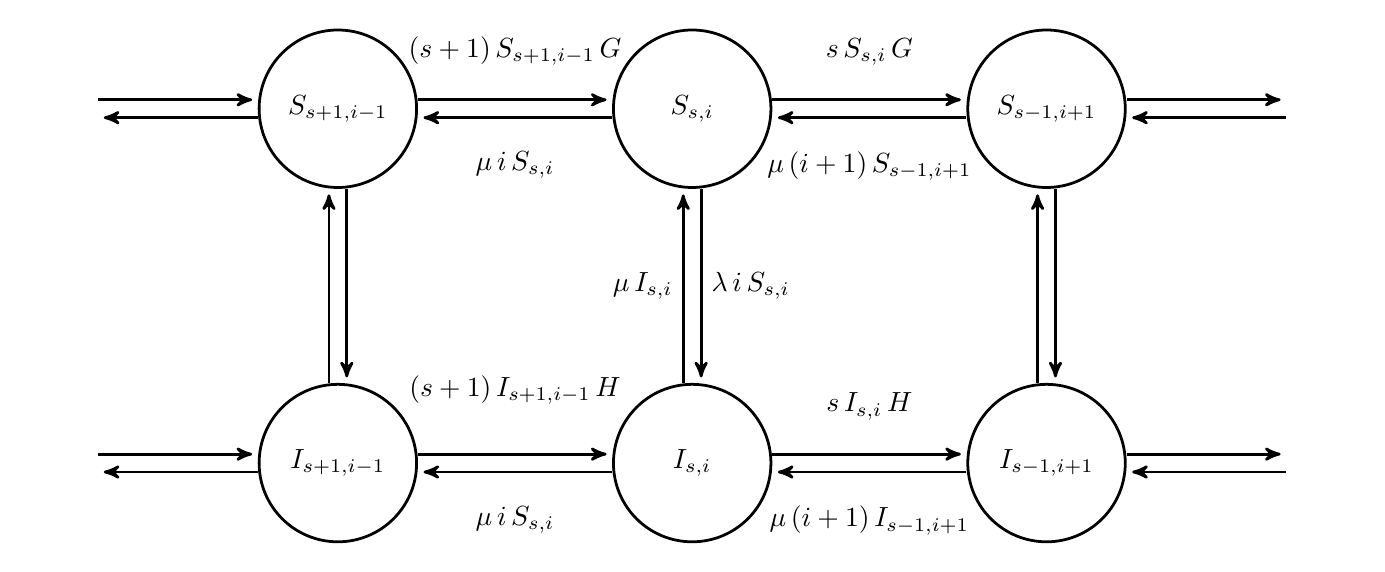
\begin{tikzpicture}[->,>=stealth',shorten >=2pt, line width=1pt, 
                                  node distance=4.5cm, ]
\node[state, minimum size=2cm] (1) at (10,0) {$S_{s,i}$};
\node[state, minimum size=2cm, left of=1] (0) {$S_{s+1,i-1}$};
\node[state, minimum size=2cm, right of=1] (2) {$S_{s-1,i+1}$};
\node[state, minimum size=2cm, below of=0] (3) {$I_{s+1,i-1}$};
\node[state, minimum size=2cm, right of=3] (4) {$I_{s,i}$};
\node[state,minimum size=2cm,right of=4] (5) {$I_{s-1,i+1}$};
\node[state,draw=none, left of=0, xshift=1cm] (hid1) {};
\node[state,draw=none, left of=3, xshift=1cm] (hid2) {};
\node[state,draw=none, right of=2, xshift=-1cm] (hid3) {};
\node[state,draw=none, right of=5, xshift=-1cm] (hid4) {};
5

\path[->, shift left=.75ex]
    (0) edge node[above=0.3cm] {$(s+1)\, S_{s+1,i-1}\, G$} (1)
    (1) edge node[below=0.3cm] {$\mu\, i\, S_{s,i}$} (0)
    (1) edge node[above=0.3cm] {$s\, S_{s,i}\, G$} (2)
    (2) edge node[below=0.3cm] {$\mu\, (i+1)\, S_{s-1,i+1}$}(1)
    (0) edge(3)
    (3) edge(0)
    (3) edge node[above=0.5cm] {$(s+1)\, I_{s+1,i-1}\, H$} (4)
    (4) edge node[below=0.3cm] {$\mu\, i\, S_{s,i}$}(3)
    (1) edge node[right] {$\lambda\, i\, S_{s,i}$} (4)
    (4) edge node[left] {$\mu\, I_{s,i}$} (1)
    (2) edge(5)
    (5) edge(2)
    (5) edge node[below=0.3cm] {$\mu\, (i+1)\, I_{s-1,i+1}$}(4)
    (4) edge node[above=0.3cm] {$s\, I_{s,i}\, H$}(5)
    (0) edge (hid1)
    (hid1) edge (0)
    (hid2) edge (3)
    (3) edge (hid2)
    (2) edge (hid3)
    (hid3) edge (2)
    (5) edge (hid4)
    (hid4) edge (5);
\end{tikzpicture}
\end{center}
\caption{Transition graph for states in Lindquist et al model} \label{fig:6.1}
\end{figure}
\clearpage

This gives the set of ODEs given by:

\begin{equation}\label{Lindquist}
\begin{split}
\frac{dS_{s,i}}{dt}=-\lambda i S_{s,i}+\mu I_{s,i} +\mu \{(i+1) S_{s-1,i+1}-iS_{s,i}\}+G\{(s+1)S_{s+1,i-1}-sS_{s,i}\}\,,\\
\frac{dI_{s,i}}{dt}=\lambda i S_{s,i}-\mu I_{s,i} +\mu \{(i+1) I_{s-1,i+1}-iI_{s,i}\}+H\{(s+1)I_{s+1,i-1}-sI_{s,i}\}\,,\\
k \in \{1,2,...,M\}
\end{split}
\end{equation}

Where $G$ and $H$ are again given by \eqref{G} and \eqref{H} respectively. Each equation has six terms represented by the six transitions in and out of each state as seen in Figure \ref{fig:6.1}. The special cases to these equations when $S_{s,i}$ is given by $S_{k,0}$ or $S_{0,k}$ or when $I_{s,i}$ is given by $I_{k,0}$ or $I_{0,k}$. In these cases the ODEs for these classes are given by:

\begin{equation}\label{Lindquist special 1}
\begin{split}
\frac{dS_{0,k}}{dt}=-\lambda k S_{0,k}+\mu I_{0,k}-\mu k S_{0,k}+G\,S_{1,k-1}\,,\\
\frac{dI_{0,k}}{dt}=\lambda k S_{0,k}-\mu I_{0,k}-\mu k I_{0,k}+H\,I_{1,k-1}\,,\\
k \in \{1,2,...,M\}
\end{split}
\end{equation}
\noindent
for the classes when the individuals have no susceptible neighbours and

\begin{equation}\label{Lindquist special 2}
\begin{split}
\frac{dS_{k,0}}{dt}=\mu I_{k,0}+\mu S_{k-1,1}-G\,kS_{k,0}\,,\\
\frac{dI_{k,0}}{dt}=\mu I_{k,0}+\mu I_{k-1,1}-H\,kI_{k,0}\,,\\
k \in \{1,2,...,M\}
\end{split}
\end{equation}
\noindent
for the classes when the individuals have no infectious neighbours. 

For every degree $k$ there are $k+1$ rate equations for the susceptible classes and $k+1$ rate equations for the infectious classes, so for each degree $k$ there are $2(k+1)$ rate equations, and if $M$ is the maximum degree in the population, this means that there are $M(M+3)$ rate equations in total for the entire system. This is a much harder system to solve than the Pastor-Satorras model outlined in Section \ref{subsec:6.1} as that model had a number of differential equations in the system to solve proportional to $M$, but this more complicated model has a number of equations proportional to $M^2$ in the system to solve.

\subsubsection{Assumptions of the Lindquist model} \label{subsub:6.2.3}

The assumptions of the Lindquist et al model are very similar to the assumptions made in the Pastor-Satorras model except one degree ``weaker''. The assumptions come in the derivation of the rates at which a neighbour of an individual is infected. First, look at the derivation of \eqref{S_s,i to S_s-1,i+1}, in which we need to find the probability that an individual in class $S_{s,i}$ is neighbour to a newly infected individual, which is given by \eqref{probSsineigh}. This assumes that all neighbours of the individuals in class $S_{s,i}$ are equally as likely to be infected where this actually depends on the degree of the neighbour. More specifically it depends on the infectious degree of the neighbour, since the more infectious neighbours an individual has, the more likely they are to be infected. This is what is meant by the assumptions being one degree ``weaker'': whereas in the Pastor-Satorras model the assumptions depended on the neighbours of individuals, in the Lindquist model the assumptions depend on the state of the neighbour's neighbour's of the individuals being examined. 

\subsection{Summary of deterministic models} \label{subsec:6.3}

In this section we have defined two deterministic models that should describe the mean behaviour of the SIS epidemic on a random network. In the next section we will investigate how well the numerical solutions of these deterministic models approximate this mean behaviour. If they are good approximations then we will investigate whether or not they remain good approximations as the parameters of the configuration model and the epidemic change, for which parameters the deterministic models give a better approximation of the mean epidemic and which model gives a better approximation, both in individual cases and overall.

\newpage
\section{Evaluation of deterministic models} \label{sec:7}

Now we have defined two deterministic models we can see how good they are at approximating the mean behaviour of an epidemic for a given prescribed degree distribution and parameters. We will also be able to see which deterministic model is a better approximation, and whether they approximate the behaviour of the mean epidemic better or worse when the parameters have certain properties such as being particularly large or small. 

In Section \ref{sec:5} we began by investigating the behaviour of the mean epidemic when the population size was $100$ individuals with $10$ of those individuals initially infectious. The prescribed degree distribution was a Poisson distribution with mean $5$ and infection rate $\lambda=1$ and recovery rate $\mu=1$ and used this as a base mean epidemic. We then changed the parameters and degree distribution of the SIS epidemic and compared how the mean epidemic of the SIS epidemic simulations then compared to the base mean epidemic. In this section we will use the same concept to investigate how well the deterministic models described in Section \ref{sec:6} approximate the mean behaviour of the epidemic. The second model that was described, the Lindquist model, is more complex as it takes more information about the population in to account and as a result we should expect this makes this model a better approximation than the Pastor-Satorras model. 

\subsection{Evaluation of models for different population scales} \label{subsec:7.1}

In Figure \ref{7.1} we can see that the both of the deterministic models approximately describe the behaviour of the mean epidemic. They both increase with the mean epidemic and find a level of stability at a value of $I(t)$ close to the value of $I(t)$ when the mean epidemic reaches a level of stability, although the Lindquist model approximated this value of $I(t)$ marginally closer than the Pastor-Satorras model. It is worth noting that since after the deterministic models reach a level of stability they stay there and since they are not random like the mean epidemic this value of $I(t)$ is at a fixed point and a stationary point for the deterministic models. However, the deterministic models do not approximate the rate at which the mean epidemic reaches the value of $I(t)$ at which the mean epidemic stabilises. Both models reach a stationary state at an earlier time than the mean epidemic reaches a level of stability, although the rate at which the Lindquist model reaches its stationary state is closer to the rate at which the mean epidemic reaches a level of stability than the Pastor-Satorras model.

\begin{figure}
\begin{center}
\includegraphics[height=10cm, width=15cm]{/Users/christianpearce/Documents/MMath/Year 4/Dissertation/Dissertation writing/SIM 100 Po5 lambda 1 mu 1 det.jpg}
\end{center}
\caption{Mean epidemic as in Figure \ref{SIM 100 Po5 lambda 1 mu 1} with Pastor-Satorras model (green) and Lindquist et al model (orange) approximations for a population size 100, 10 individuals initially infected, Poisson degree distribution $\overline{k}=5$, $\lambda=1$, $\mu=1$.}
\label{7.1}
\end{figure}

Comparing Figure \ref{7.1} to Figure \ref{7.2} we can see that both deterministic models still closely approximate the behaviour of the mean epidemic but when the population size is increased and the proportion of the population which is initially infectious stays the same, the mean epidemic approaches the Lindquist model, making the behaviour of the mean epidemic almost exactly the behaviour of the Lindquist model. The implication of this is that the deterministic models describe the asymptotic behaviour of the mean epidemic better as $N\rightarrow\infty$ where $N$ is the size of the population.

\begin{figure}
\begin{center}
\includegraphics[height=10cm, width=15cm]{/Users/christianpearce/Documents/MMath/Year 4/Dissertation/Dissertation writing/n1000 SIM 100 Po5 lambda 1 mu 1 det.jpg}
\end{center}
\caption{Mean epidemic as in Figure \ref{n1000 SIM 100 Po5 lambda 1 mu 1} with Pastor-Satorras model (green) and Lindquist et al model (orange) approximations for a population size 1000, 100 individuals initially infected, Poisson degree distribution $\overline{k}=5$, $\lambda=1$, $\mu=1$.}
\label{7.2}
\end{figure}

\subsection{Evaluation of models for different infection and recovery rates} \label{subsec:7.2}

Next, we investigated the influence on the behaviour of the mean epidemic when the values of the infection rate $\lambda$ and the recovery rate $\mu$ were changed. As we can see from Figure \ref{7.3}, both the Lindquist and the Pastor-Satorras models approximate the mean epidemic very well when the value of $\lambda$ is changed from $1$ to $10$. They both still approximate that the mean epidemic will take off and become established in the population and both reach a stationary state at a value of $I(t)$ very close to the value of $I(t)$ where the mean epidemic finds a level of stability. As well as this both deterministic models reach a stationary state at a time very close to the time that the mean epidemic reaches a level of stability. What is more, both deterministic models follow virtually the same line so in this case it is very difficult to distinguish which deterministic model is a better approximator, although they are both very good approximators.

\begin{figure}
\begin{center}
\includegraphics[height=10cm, width=15cm]{/Users/christianpearce/Documents/MMath/Year 4/Dissertation/Dissertation writing/SIM 100 Po5 lambda 10 mu 1 det.jpg}
\end{center}
\caption{Mean epidemic as in Figure \ref{SIM 100 Po5 lambda 10 mu 1} with Pastor-Satorras model (green) and Lindquist et al model (orange) approximations for a population size 100, 10 individuals initially infected, Poisson degree distribution $\overline{k}=5$, $\lambda=10$, $\mu=1$.}
\label{7.3}
\end{figure}

When the value of $\mu$ is changed from $1$ to $10$, we know that the mean epidemic now does not take off and instead goes extinct. In this case, as we can see in Figures \ref{7.4} and \ref{7.5} both deterministic models also approximate that the mean epidemic goes extinct. Both deterministic models also follow virtually the same line and are almost indistinguishable when superimposed. This means that in this case both deterministic models are very good approximators of the mean behaviour of the epidemic and neither can be considered to be a better approximator than the other. 

\begin{figure}
\begin{center}
\includegraphics[height=10cm, width=15cm]{/Users/christianpearce/Documents/MMath/Year 4/Dissertation/Dissertation writing/SIM 100 Po5 lambda 1 mu 10 det.jpg}
\end{center}
\caption{Mean epidemic as in Figure \ref{SIM 100 Po5 lambda 1 mu 10} with Pastor-Satorras model approximation for a population size 100, 10 individuals initially infected, Poisson degree distribution $\overline{k}=5$, $\lambda=1$, $\mu=10$.}
\label{7.4}
\end{figure}

\begin{figure}
\begin{center}
\includegraphics[height=10cm, width=15cm]{/Users/christianpearce/Documents/MMath/Year 4/Dissertation/Dissertation writing/SIM 100 Po5 lambda 1 mu 10 det 2.jpg}
\end{center}
\caption{Mean epidemic as in Figure \ref{SIM 100 Po5 lambda 1 mu 10} with Lindquist et al model (orange) approximation for a population size 100, 10 individuals initially infected, Poisson degree distribution $\overline{k}=5$, $\lambda=1$, $\mu=10$.}
\label{7.5}
\end{figure}

Figure \ref{7.6} shows the mean behaviour of the epidemic when the values of $\lambda$ and $\mu$ are both changed but kept in the same proportion to one another. As we can see, both deterministic models take off and become established in the population, as does the mean epidemic. Both deterministic models reach a stationary state at a value of $I(t)$ close to the value of $I(t)$ the mean epidemic takes when it reaches a level of stability, although the Lindquist model approximates this value more closely than the Pastor-Satorras model. However, both deterministic models reach a stationary state at much more quickly than the mean epidemic reaches a level of stability and so do not approximate the rate at which the mean epidemic reaches a level of stability very well, although the Lindquist model approximates this rate closer than the Pastor-Satorras model. In summary, both deterministic models are a good approximation for the mean behaviour of the epidemic but, are much better approximators when the infection rate $\lambda$ and the recovery rate $\mu$ are more out of proportion with one another. Out of the two deterministic models we have described, in these cases, the Lindquist model seems to be better at approximating the mean behaviour of the epidemic.

\begin{figure}
\begin{center}
\includegraphics[height=10cm, width=15cm]{/Users/christianpearce/Documents/MMath/Year 4/Dissertation/Dissertation writing/SIM 100 Po5 lambda 10 mu 10 det.jpg}
\end{center}
\caption{Mean epidemic as in Figure \ref{SIM 100 Po5 lambda 10 mu 10} with Pastor-Satorras model (green) and Lindquist et al model (orange) approximations for a population size 100, 10 individuals initially infected, Poisson degree distribution $\overline{k}=5$, $\lambda=10$, $\mu=10$.}
\label{7.6}
\end{figure}

\subsection{Evaluation of models for different degree distribution mean} \label{subsec:7.3}

Now consider the cases where the mean of the prescribed degree distribution was changed. First, we saw the effect on the mean epidemic when the mean was made large. As we can see from Figure \ref{7.7}, when the mean of the degree distribution is made large, both deterministic models take off as does the mean epidemic, and initially they both increase at the same rate as each other and the mean epidemic. However, both deterministic models reach a stationary value at a smaller value of $I(t)$ than the value of $I(t)$ at which the mean epidemic reaches a level of stability. As well as this both deterministic models reach a stationary value at the same value of $I(t)$ and follow virtually the same line so neither deterministic model is a better approximation in this case.

\begin{figure}
\begin{center}
\includegraphics[height=10cm, width=15cm]{/Users/christianpearce/Documents/MMath/Year 4/Dissertation/Dissertation writing/SIM 100 Po10 lambda 1 mu 1 det.jpg}
\end{center}
\caption{Mean epidemic as in Figure \ref{SIM 100 Po10 lambda 1 mu 1} with Pastor-Satorras model (green) and Lindquist et al model (orange) approximations for the a population size 100, 10 individuals initially infected, Poisson degree distribution $\overline{k}=10$, $\lambda=1$, $\mu=1$.}
\label{7.7}
\end{figure}

As we can see in Figure \ref{7.8}, when the mean of the degree distribution is decreased, both deterministic models take off, as does the mean epidemic. However, the Pastor-Satorras model increases at a faster rate than the mean epidemic and reaches a stationary state at a much higher value of $I(t)$ than the value of $I(t)$ at which the mean epidemic reaches a level of stability. The Lindquist model also takes off and becomes established in the population like the mean epidemic, increases more quickly than the mean epidemic and reaches a stationary state at a larger value of $I(t)$ than the value of $I(t)$ at which the mean epidemic reaches a level of stability. However, the Lindquist model increases at a rate and settles at a value of $I(t)$ closer to that of the mean epidemic. So, in this case neither deterministic model is a particularly good approximation of the mean epidemic but, the Lindquist model is a better approximation than the Pastor-Satorras model.

\begin{figure}
\begin{center}
\includegraphics[height=10cm, width=15cm]{/Users/christianpearce/Documents/MMath/Year 4/Dissertation/Dissertation writing/SIM 100 Po2 lambda 1 mu 1 det.jpg}
\end{center}
\caption{Mean epidemic as in Figure \ref{SIM 100 Po2 lambda 1 mu 1} with Pastor-Satorras model (green) and Lindquist et al model (orange) approximations for a population size 100, 10 individuals initially infected, Poisson degree distribution $\overline{k}=2$, $\lambda=1$, $\mu=1$.}
\label{7.8}
\end{figure}

\subsection{Evaluation of models for different values of $\frac{\mu}{\lambda}=\overline{k}$} \label{subsec:7.4}

Next, we investigated the behaviour of the mean epidemic when multiple parameters were changed to change the relationship between them. In Figure \ref{7.9} the mean of the degree distribution was changed to $2$ and the recovery rate $\mu$ was increased to $3$ so that $\frac{\mu}{\lambda}>\overline{k}$ where $\overline{k}$ is the mean of the degree distribution. In this case both deterministic models go to $0$ quickly like the mean epidemic and the Lindquist model approaches $0$ at approximately the same rate as the mean epidemic, however, the Pastor-Satorras model approaches $0$ at a much slower rate. Therefore, in this case the Lindquist model can be considered a good approximation for the mean epidemic and the Pastor-Satorras model is not a good approximation.

\begin{figure}
\begin{center}
\includegraphics[height=10cm, width=15cm]{/Users/christianpearce/Documents/MMath/Year 4/Dissertation/Dissertation writing/SIM 100 Po 2 lambda 1 mu 3 det.jpg}
\end{center}
\caption{Mean epidemic as in Figure \ref{SIM 100 Po2 lambda 1 mu 3} with Pastor-Satorras model (green) and Lindquist et al model (orange) approximations for a population size 100, 10 individuals initially infected, Poisson degree distribution $\overline{k}=2$, $\lambda=1$, $\mu=3$.}
\label{7.9}
\end{figure}

Figure \ref{7.10} shows the mean epidemic when $\overline{k}$ was decreased to $3$ and the values of the infection rate and recovery rate $\mu$ were changed to $4$ and $12$ respectively so that $\frac{\mu}{\lambda}=\overline{k}$. As mentioned in Section \ref{sec:5}, the values of $\lambda$ and $\mu$ will have little effect on the shape of the mean epidemic except for the rate at which $I(t)$ increases or decreases so when considering the behaviour of the mean epidemic when $\frac{\mu}{\lambda}=\overline{k}$ the size of $\lambda$ and $\mu$ does not matter. Whereas before both deterministic models generally behave the same, in this case the Pastor-Satorras model takes off and the Lindquist model does not. Therefore, it is immediately obvious that in this case the Pastor-Satorras model is not a good approximation of the mean epidemic.

\begin{figure}
\begin{center}
\includegraphics[height=10cm, width=15cm]{/Users/christianpearce/Documents/MMath/Year 4/Dissertation/Dissertation writing/SIM 100 Po3 lambda 4 mu 12 det.jpg}
\end{center}
\caption{Mean epidemic as in Figure \ref{SIM 100 Po3 lambda 4 mu 12} with Pastor-Satorras model (green) and Lindquist et al model (orange) approximations for a population size 100, 10 individuals initially infected, Poisson degree distribution $\overline{k}=3$, $\lambda=4$, $\mu=12$.}
\label{7.10}
\end{figure}

Figure \ref{7.11} shows the approximations of the Pastor-Satorras and Lindquist models when $\frac{\mu}{\lambda}=\overline{k}$ but the mean of the degree distribution is high along side the mean epidemic for this case. As we can see, this time the value of $I(t)$ decreases for both deterministic models, as does the mean epidemic. Both deterministic models decrease at a rate slower than the mean epidemic however the Pastor-Satorras model reaches a stationary state at a larger value of $I(t)$ than the mean epidemic whereas the Lindquist model begins to behave more like the mean epidemic after some time. In summary, when we approximately have $\frac{\mu}{\lambda}=\overline{k}$ the Lindquist model is a better approximation for the mean epidemic than the Pastor-Satorras model.

\begin{figure}
\begin{center}
\includegraphics[height=10cm, width=15cm]{/Users/christianpearce/Documents/MMath/Year 4/Dissertation/Dissertation writing/SIM 100 Po8 lambda 1 mu 8 det.jpg}
\end{center}
\caption{Mean epidemic as in Figure \ref{SIM 100 Po8 lambda 1 mu 8} with Pastor-Satorras model (green) and Lindquist et al model (orange) approximations for a population size 100, 10 individuals initially infected, Poisson degree distribution $\overline{k}=8$, $\lambda=1$, $\mu=8$.}
\label{7.11}
\end{figure}

\subsection{Evaluation of models for different prescribed degree distribution} \label{subsec:7.5}

Finally, Figure \ref{7.12} shows the approximations of the Pastor-Satorras and Lindquist models when the configuration model is constructed using a Geometric distribution instead of Poisson distribution, which is a distribution that is not as concentrated around the mean and has a tail which decays at a slower rate. In this final case both deterministic models take off as does the mean epidemic and both reach a stationary state at approximately the same value of $I(t)$ at which the mean epidemic reaches a level of stability. What is more, both deterministic models approach this value of $I(t)$ at approximately the same rate as the mean epidemic. The only difference between the approximations of the deterministic models in this case is that the value of $I(t)$ at which the Lindquist model reaches a stationary state is a marginally closer to the value of value of $I(t)$ at which the mean epidemic reaches a level of stability than the value of $I(t)$ at which the Pastor-Satorras model reaches a stationary state. 

As well, in this case the deterministic models approximate the mean epidemic much closer than when the parameters are the same, however, the prescribed degree distribution is a Poisson distribution.  Therefore, in this case we can say that both deterministic models are a good approximation for the mean epidemic, but the Lindquist model is a better approximation.

\begin{figure}
\begin{center}
\includegraphics[height=10cm, width=15cm]{/Users/christianpearce/Documents/MMath/Year 4/Dissertation/Dissertation writing/SIM 100 Geom5 lambda 1 mu 1 det.jpg}
\end{center}
\caption{Mean epidemic as in Figure \ref{SIM 100 Geom5 lambda 1 mu 1} with Pastor-Satorras model (green) and Lindquist et al model (orange) approximations for the a population size 100, 10 individuals initially infected, Geometric degree distribution $\overline{k}=5$, $\lambda=1$, $\mu=1$.}
\label{7.12}
\end{figure}

\subsection{Summary of evaluation of deterministic models} \label{subsec:7.6}

In this section we have compared the solutions of two deterministic models, the Pastor-Satorras model and the Lindquist model, to the mean behaviour of the SIS epidemic on a random network for several cases of varying parameters. Both models closely approximated the mean epidemic in most cases but in every case the Lindquist model approximated the behaviour of the mean epidemic more closely. However, there were cases when the Lindquist model was not as good of an approximation. When the relationship between the infection rate $\lambda$, the recovery rate $\mu$ and the mean of the prescribed degree distribution $\overline{k}$ is approximately $\frac{\mu}{\lambda}=\overline{k}$ then both models were not as good approximations for the behaviour of the mean epidemic. As well as this, when the value of $\overline{k}$ was small then both models were not good approximations of the mean behaviour of the epidemic. We also found that when the prescribed degree distribution was changed from a Poisson distribution to a Geometric distribution then the deterministic models were much closer approximations of the mean epidemic. And finally the deterministic models were much better approximations of the mean epidemic when $N \rightarrow \infty$.

\newpage
\section{Conclusion} \label{sec:8}

The purpose of this report has been to describe the SIS epidemic on a random network in depth and investigate its behaviour and then investigate how is best to approximate its mean behaviour. In Section \ref{sec:4} we described the properties and behaviour of the real epidemic and streamlined it into an idealised version that could be described mathematically. In Section \ref{sec:5} we then rigorously defined the two parts of the mathematical model: the configuration model and the SIS epidemic, and the theory that goes with them. As well we saw how the SIS epidemic on random network behaves.

We have simulated the SIS epidemic on a random network as a random stochastic process and found its mean behaviour. We have found that this behaviour changes depending on the parameters of the prescribed degree distribution and the SIS epidemic itself. These parameters are: the size of the population $N$, the probability distribution used for the prescribed degree distribution, the mean of the prescribed degree distribution $\overline{k}$, the infection rate $\lambda$ and the recovery rate $\mu$. We found that the mean behaviour of the epidemic either took off and the infection became established in the population or the infection went extinct quickly and this depended on the relationship between $\lambda$, $\mu$ and $\overline{k}$. If $\frac{\mu}{\lambda}>\overline{k}$ then it was likely that the infection will become extinct whereas if $\frac{\mu}{\lambda}<\overline{k}$ then the infection takes off and the number of infectious individuals in the population $I(t)$ increases until it reaches a certain value and then levels off. It was found that this value of $I(t)$ is heavily dependent on the ratio of the infection rate $\lambda$ and the recovery rate $\mu$ and also on the size of $\overline{k}$. As the ratio of the infection rate $\lambda$ and the recovery rate $\mu$ increased, so did this value of $I(t)$. As well, as $\overline{k}$ increased, so did this value of $I(t)$. As well as this, when the prescribed degree distribution is changed from a Poisson distribution to a Geometric distribution, a probability distribution with a heavier tail making it not as concentrated around the mean, this value of $I(t)$ also decreased in this case. This could be due to that there are more individuals with a small number of neighbours, so the effect is similar to when the mean of the degree distribution is decreased.

We can also approximate this behaviour by using deterministic models. In this report two deterministic models have been defined with the aim of approximating the mean behaviour of the epidemic defined in Section \ref{sec:6}. The first, simpler model is the model proposed by Pastor-Satorras and Vespignani in 2001 \cite{bibpastor}. This model describes the proportion of individuals with degree $k$ who are infected through time, for $k \in \{1,2,…,M\}$ where $M$ is the maximum degree of the population. The system of differential equations that make up this model are given by \eqref{Pastor-Satorras} and \eqref{Pastor sum} The second, more complicated model is the model proposed by Lindquist et al in 2011 \cite{biblindquist}. This model describes the number of infected individuals and the number of infected individuals who have degree $k$ through time as well as the number of each individual’s neighbours who are susceptible or infectious. The system of differential equations that make up this model are given by \eqref{Lindquist} as well as the special cases given by \eqref{Lindquist special 1} and \eqref{Lindquist special 2}.

When compared with the mean simulations of the epidemic, both models provided a fair approximation in most cases, however, in every case the Lindquist model was a better approximation. There were also some situations in which the deterministic models were better approximations than others. In one case when the relationship was $\frac{\mu}{\lambda}=\overline{k}$ between the infection rate $\lambda$, the recovery rate $\mu$ and the mean of the prescribed degree distribution then the Pastor-Satorras model a took off whereas the simulated epidemic tended towards $0$ which the Lindquist model also did. However, despite this the Lindquist model was not as good of an approximation for the mean behaviour of the epidemic as in other cases.

As well as this, when the simulations use a Poisson degree distribution and $\lambda$ and $\mu$ are approximately equal then both deterministic models are not as good approximations of the mean behaviour of the epidemic. Both models reach a stationary state when approximately the same proportion of the population is infectious as the proportion of the population that is infectious when the mean behaviour of the epidemic reaches a level of stability, but both models reach this proportion much more quickly than the mean epidemic, so in this case were not as good approximations.

In summary, we have successfully found deterministic approximations for the SIS epidemic on a random network and found out in what cases they are better and worse approximations. In future work it would be interesting to explore the effect of further degree distributions on the mean behaviour of the epidemic besides Poisson and Geometric distributions such as a Power law distribution which has a heavier tail than a Geometric and Poisson distribution. As well as this, most of the cases in this report have only investigated the effect that changing one parameter of the mathematical model has on the mean behaviour of the epidemic. Therefore, future work could include investigating the effect that changing more combinations of the model parameters and changing the parameters of the model under a different degree distribution has on the mean behaviour of the epidemic and the accuracy of the approximations of the deterministic models in these cases.

As well, the deterministic models are used as an approximation of an idealised model which itself is an approximation of a real epidemic. This means that it is likely that a real epidemic could act much differently to the simulations detailed in this report. This could lead more ambitious future studies which investigate the effect of including different types of social structures in the configuration model and how that would affect the behaviour of the mean epidemic and the deterministic models. It would be interesting to consider what effect friend groups or families being included in the population and individual infection rates between pairs of individuals, so the random network would have weighted edges to represent the different rates at which individuals interact instead of assuming an individual contacts all of its neighbours at the same rate constant rate $\lambda$, have on this behaviour. A more complicated characteristic of the epidemic to include might be unique iid but not exponentially distributed infection times. Since in a real epidemic the length of time you have left to be infectious will depend heavily on how long you have been infected for and the treatment you have received whereas in a Poisson process it does not.

\newpage
\listoffigures

\newpage
\begin{thebibliography}{99} % alternatively use BibTeX

\bibitem{bibandersson1}
H. ~Andersson,
{\it Epidemic Models and Social Networks\/},
The Mathematical Scientist Vol.~24, 
128--147
(1999).

\bibitem{bibandersson2}
H. ~Andersson,
{\it Limit Theorems for a Random Graph Epidemic Model\/},
The Annals of Applied Probability,
 Vol. 8, No. 4, 1331--1349 
(1998).

\bibitem{bibandersson3}
H. ~Andersson, T. ~Britton,
{\it Stochastic Epidemic Models and their Statistical Analysis\/},
Springer,
(2000).

\bibitem{bibbollobas}
B. ~Bollob$\acute{a}$s,
{\it Random Graphs\/}, 
Harcourt Brace Jovanovich,
(1985).

\bibitem{bibbritton}
T. ~Britton, M. ~Deijfen, A. ~Martin-Löf,
{\it Generating Simple Random Graphs with Prescribed Degree Distribution\/},
Journal of Statistical Physics,
 Vol. 124, No. 6, 1377–1397 
(2006).

\bibitem{bibbryson}
M. ~Bryson,
{\it Heavy Tailed Distributions: Properties and Tests\/},
Technometrics,
 Vol. 16, No. 1, 61--68 
(1974).

\bibitem{bibgray}
A. ~Gray, D. ~Greenhalgh, L. ~Hu, X. ~Mao, J. ~Pan,
{\it A Stochastic Differential Equation SIS Epidemic Model\/},
SIAM Journal on Applied Mathematics,
 Vol. 71, No. 3, 876–902 
(2011).

\bibitem{bibhiebeler}
D. ~Hiebeler, R. ~Rier, J. ~Audibert, P. ~LeClair, A. ~Webber,
{\it Variability in a Community-Structured SIS Epidemiological Model\/},
Bulletin of Mathematical Biology,
 Vol. 77, No. 4, 698–712 
(2015).

\bibitem{bibkephart}
J. ~O. Kephart, S. ~R. White, 
{\it Directed-Graph Epidemiological Models of Computer Viruses\/},
Proceedings. 1991 IEEE Computer Society Symposium on Research in Security and Privacy,
(1991).

\bibitem{bibliljeros}
F. ~Liljeros, C. ~R. Edling, L. ~A. Nunes Amaral, H. ~Eugene Stanley, Y. ~Åberg,
{\it The web of human sexual contacts\/},
Nature,
 Vol. 411, No. 6840, 907 
(2015).

\bibitem{biblindquist}
J. ~Lindquist, J. ~Ma, P. ~van den Driessche, F. ~Willeboorsde,
{\it Effective Degree Network Disease Models\/},
Journal of Mathematical Biology,
 Vol. 62, No. 2, 143--164
(2011).

\bibitem{bibpan}
J. ~Pan, A. ~Gray, D. ~Greenhalgh, X. ~Mao,
{\it Parameter Estimation for the Stochastic SIS Epidemic Model\/},
Statistical Inference for Stochastic Processes,
 Vol. 17, No. 1, 75--98
(2014).

\bibitem{bibpastor}
R. ~Pastor-Satorras, A. ~Vespignani,
{\it Epidemic Spreading in Scale-Free Networks\/},
Physical review letters,
 Vol. 86, No. 14, 3200--3203
(2001).

\bibitem{bibyang}
L. ~Yang, X. ~Yang,
{\it The Spread of Computer Viruses Over a Reduced Scale-Free Network\/},
Physica A: Statistical Mechanics and its Applications,
 Vol. 396, 173--184
(2014).

\bibitem{bibyorke}
A. ~J. Yorke, H. ~W. Hethcote, A. ~W. Nold
{\it Dynamics and Control of the Transmission of Gonorrhea\/},
Sexually Transmitted Diseases,
 Vol. 5, No. 2, 51--56
(1978).


\end{thebibliography}

\end{document}